\documentclass[a4paper]{article}

\usepackage[english]{babel}
\usepackage[latin1]{inputenc}
\usepackage{amssymb}
\usepackage{framed}
\usepackage{graphicx}
\usepackage{float}
\usepackage{subcaption}
\usepackage{mwe}
\graphicspath{ {./img/} }

\setlength{\parindent}{0pt}
\setlength{\parskip}{3ex}

\begin{document}

\begin{center}
  {\large Artificial Neural Networks and Deep Architectures, DD2437}\\
  \vspace{7mm}
  {\huge Short report on lab assignment 1\\[1ex]}
  {\Large Learning and generalisation in feed-forward networks ---\\[1ex]
 from perceptron learning to backprop}\\
  \vspace{8mm}  
  {\Large Etienne Jodry, Frano Rajic, Ivan Stresec\\}
  \vspace{4mm}
  {\large September 9, 2020\\}
\end{center}

%\begin{framed}
%Please be aware of the constraints for this document. The main intention here is that you learn how to select and organise the most relevant information into a concise and coherent report. The upper limit for the number of pages is 6 with fonts and margins comparable to those in this template and no appendices are allowed. \\
%These short reports should be submitted to Canvas by the authors as a team before the lab presentation is made. To claim bonus points the authors should uploaded their short report a day before the bonus point deadline. The report can serve as a support for your lab presentation, though you may put emphasis on different aspects in your oral demonstration in the lab.
%Below you find some extra instructions in italics. Please remove them and use normal font for your text.
%\end{framed}

\section{Main objectives and scope of the assignment}

%\textit{List here a concise list of your major intended goals, what you planned to do and what you wanted to learn/what problems you were set to address or investigate, e.g.}\\
Our major goals in the assignment were  
\begin{itemize}
    \item to implement and understand the perceptron, delta, and generalised delta learning rules
    \item to implement single- and multi-layer networks and observe their performance in relation to various hyperparameters
    \item to apply networks in solving problems of classification, encoding, and regression
    \item to use multi-layered networks in time-series predictions and observe the influence of regularization and noisy data sets on performance
    %\item to recognize risks associated with backpropagation and minimize them for robust learning of multi-layer perceptrons
    %\item to configure and monitor the behavior of learning algorithms for single- and multi-layer perceptrons networks
    %\item to identify key limitations of single-layer networks
    %\item to design and apply networks in classification, function approximation and generalisation tasks
\end{itemize}

%\textit{Then you can write two or three sentences about the scope, limitations and assumptions made for the lab assignment}
% In this lab we implemented single- and multi-layer perceptrons with focus
% on the associated learning algorithms. Furthermore, we studied their properties by
% means of simulations.

In the first part of the lab, the focus was on the Delta rule and the generalized Delta rule for two-layer perceptrons.
We designed neural networks for classification, data compression, and function approximation.

In the second part of the lab assignment we worked with multi-layer perceptrons to predict the Mackey-Glass time series. In this task we designed and evaluated the neural
networks with the ambition of delivering a robust solution with good generalization capabilities. % For this purpose, we exploited sckit-learn and TensorFlow libraries in Python.

\section{Methods}
%\textit{Mention here in just a couple of sentences what tools you have used, e.g. programming/scripting environment, toolboxes. If you use some unconventional method or introduce a clearly different performance measure, you can briefly mention or define it here.}\\
We used Python 3.8 with the PyCharm IDE. Python libraries used include numpy, matplotlib, and TensorFlow. % and scikit-learn. % We used GitHub to version the software.


\section{Results and discussion - Part I}

%
\subsection{Classification with a single-layer perceptron} \label{section_slp} % \textit{(ca.1 page)}
%
On linearly separable data we reached 100\% accuracy with both the perceptron (PR) and the delta learning rule (DR), in either batch or sequential mode. PR converges faster than DR, as it takes more time for the latter to minimize loss when maximal accuracy is already achieved.
%
%
%
For DR, the best learning rate for batch mode is around $\eta = 0.002$ and above that value it tends to diverge. Sequential converges faster with a learning rate on the whole range between $0.0001$ and $0.2$, although it has a much higher loss.
%
Convergence speed is very sensitive on the initial weights for sequential as opposed to batch learning, which is not. %, whereas for batch learning it is not very sensitive. % TODO check
%
\begin{table}[H]
	\centering
	\caption{Perceptron learning rule}
	\label{tab:pcn}
	\resizebox{\textwidth}{!}{%
		\begin{tabular}{|l|r|r|r|r|r|r|r|}
			\hline
			Learning rate            & 0.001    & 0.005    & 0.01     & 0.1      & 0.25     & 1        & 10       \\ \hline
			Accuracy - mean          & 100.00\% & 100.00\% & 100.00\% & 100.00\% & 100.00\% & 100.00\% & 100.00\% \\ \hline
			%Accuracy - std           & 0.00\%   & 0.00\%   & 0.00\%   & 0.00\%   & 0.00\%   & 0.00\%   & 0.00\%   \\ \hline
			Convergence epoch - mean & 29.22    & 8.26     & 3.45     & 1.91     & 1.90     & 1.93     & 1.87     \\ \hline
			Convergence epoch - std  & 27.84    & 6.80     & 2.14     & 0.38     & 0.30     & 0.32     & 0.42     \\ \hline
		\end{tabular}%
	}
\end{table}
\begin{table}[H]
	\centering
	\caption{Batch delta learning rule}
	\label{tab:pcn_delta_batch}
	\resizebox{\textwidth}{!}{%
		\begin{tabular}{|l|r|r|r|r|r|r|r|}
			\hline
                Learning rate            & 0.0001   & 0.001    & 0.002    & 0.003    & 0.004    & 0.005    & 0.01     \\ \hline
                Accuracy - mean          & 100.00\% & 100.00\% & 100.00\% & diverged & diverged & diverged & diverged \\ \hline
                %Accuracy - std           & 0.00\%   & 0.00\%   & 0.00\%   & 0.00\%   & 0.00\%   & 0.00\%   & 0.00\%   \\ \hline
                Convergence epoch - mean & 1,081.97 & 110.99   & 117.69   & diverged     & diverged     & diverged     & diverged     \\ \hline
                Convergence epoch - std  & 245.30   & 25.02    & 16.39    & diverged     & diverged     & diverged     & diverged     \\ \hline
                MSE Loss - mean          & 5.81E-02 & 5.81E-02 & 5.81E-02 & diverged & diverged & diverged & diverged \\ \hline
                MSE Loss - std           & 3.54E-07 & 1.51E-07 & 7.67E-08 & diverged & diverged & diverged & diverged \\ \hline
		\end{tabular}%
	}
\end{table}
\begin{table}[H]
\centering
\caption{Sequential delta learning rule}
\label{tab:pcn_delta_seq}
\resizebox{\textwidth}{!}{%
\begin{tabular}{|l|r|r|r|r|r|r|r|}
\hline
Learning rate                  & 0.0001   & 0.001    & 0.002    & 0.003    & 0.004    & 0.005    & 0.01  \\ \hline
Accuracy - mean  & 100.00\% & 100.00\% & 100.00\% & 100.00\% & 100.00\% & 100.00\% & 100.00\%  \\ \hline
% Accuracy - std   & 0.00\%   & 0.00\%   & 0.00\%   & 0.00\%   & 0.00\%   & 0.00\%   & 0.00\%   \\ \hline
Convergence epoch - mean & 1,009.25 & 108.69   & 70.43    & 58.63    & 51.19    & 61.08    & 49.02   \\ \hline
Convergence epoch - std  & 250.40   & 34.33    & 36.30    & 29.41    & 31.78    & 39.73    & 33.77    \\ \hline
MSE Loss - mean      & 6.24E+00 & 5.83E+00 & 5.83E+00 & 5.82E+00 & 5.82E+00 & 5.81E+00 & 5.84E+00 \\ \hline
MSE Loss - std       & 4.24E+00 & 4.09E-03 & 1.28E-02 & 2.39E-02 & 3.23E-02 & 3.67E-02 & 4.83E-02 \\ \hline
\end{tabular}%
}
\end{table}
Bias represents how distant the linear separator is from the origin; DR with no bias weights can result in successful separation of classes if a separating line can be drawn through the origin, and unsuccessful if not.\\
% We used inseparable two-class datasets to train batch learning with various ways of subsampling the data to see the resulting effect on performance and boundary line position. In context of uneven class representation, the line will be drawn in such a way that the more frequent class gets higher individual accuracy. In context of non-representative class distribution, we came across a case where one part of the non-representative class was entirely disregarded and falsely classified as the opposite class by the decision boundary.
We subsampled the non-linearly separable data in various ways to see the effects on performances and decision boundaries. With uneven class representation, the drawn line penalizes the minority class. We came across a case where one part of the non-representative class was entirely misclassified by the model.
% The resulting decision boundaries for 4 different subsamples of the dataset are shown in figure \ref{fig:inseparable_datasets_lines}.
In all subsampling cases, we noticed that measured accuracy on the original dataset  was lower, which means that both unrepresentative sample distribution and uneven class representation decrease the generalization capability of the trained model.
%\begin{figure}
%	\centering
%	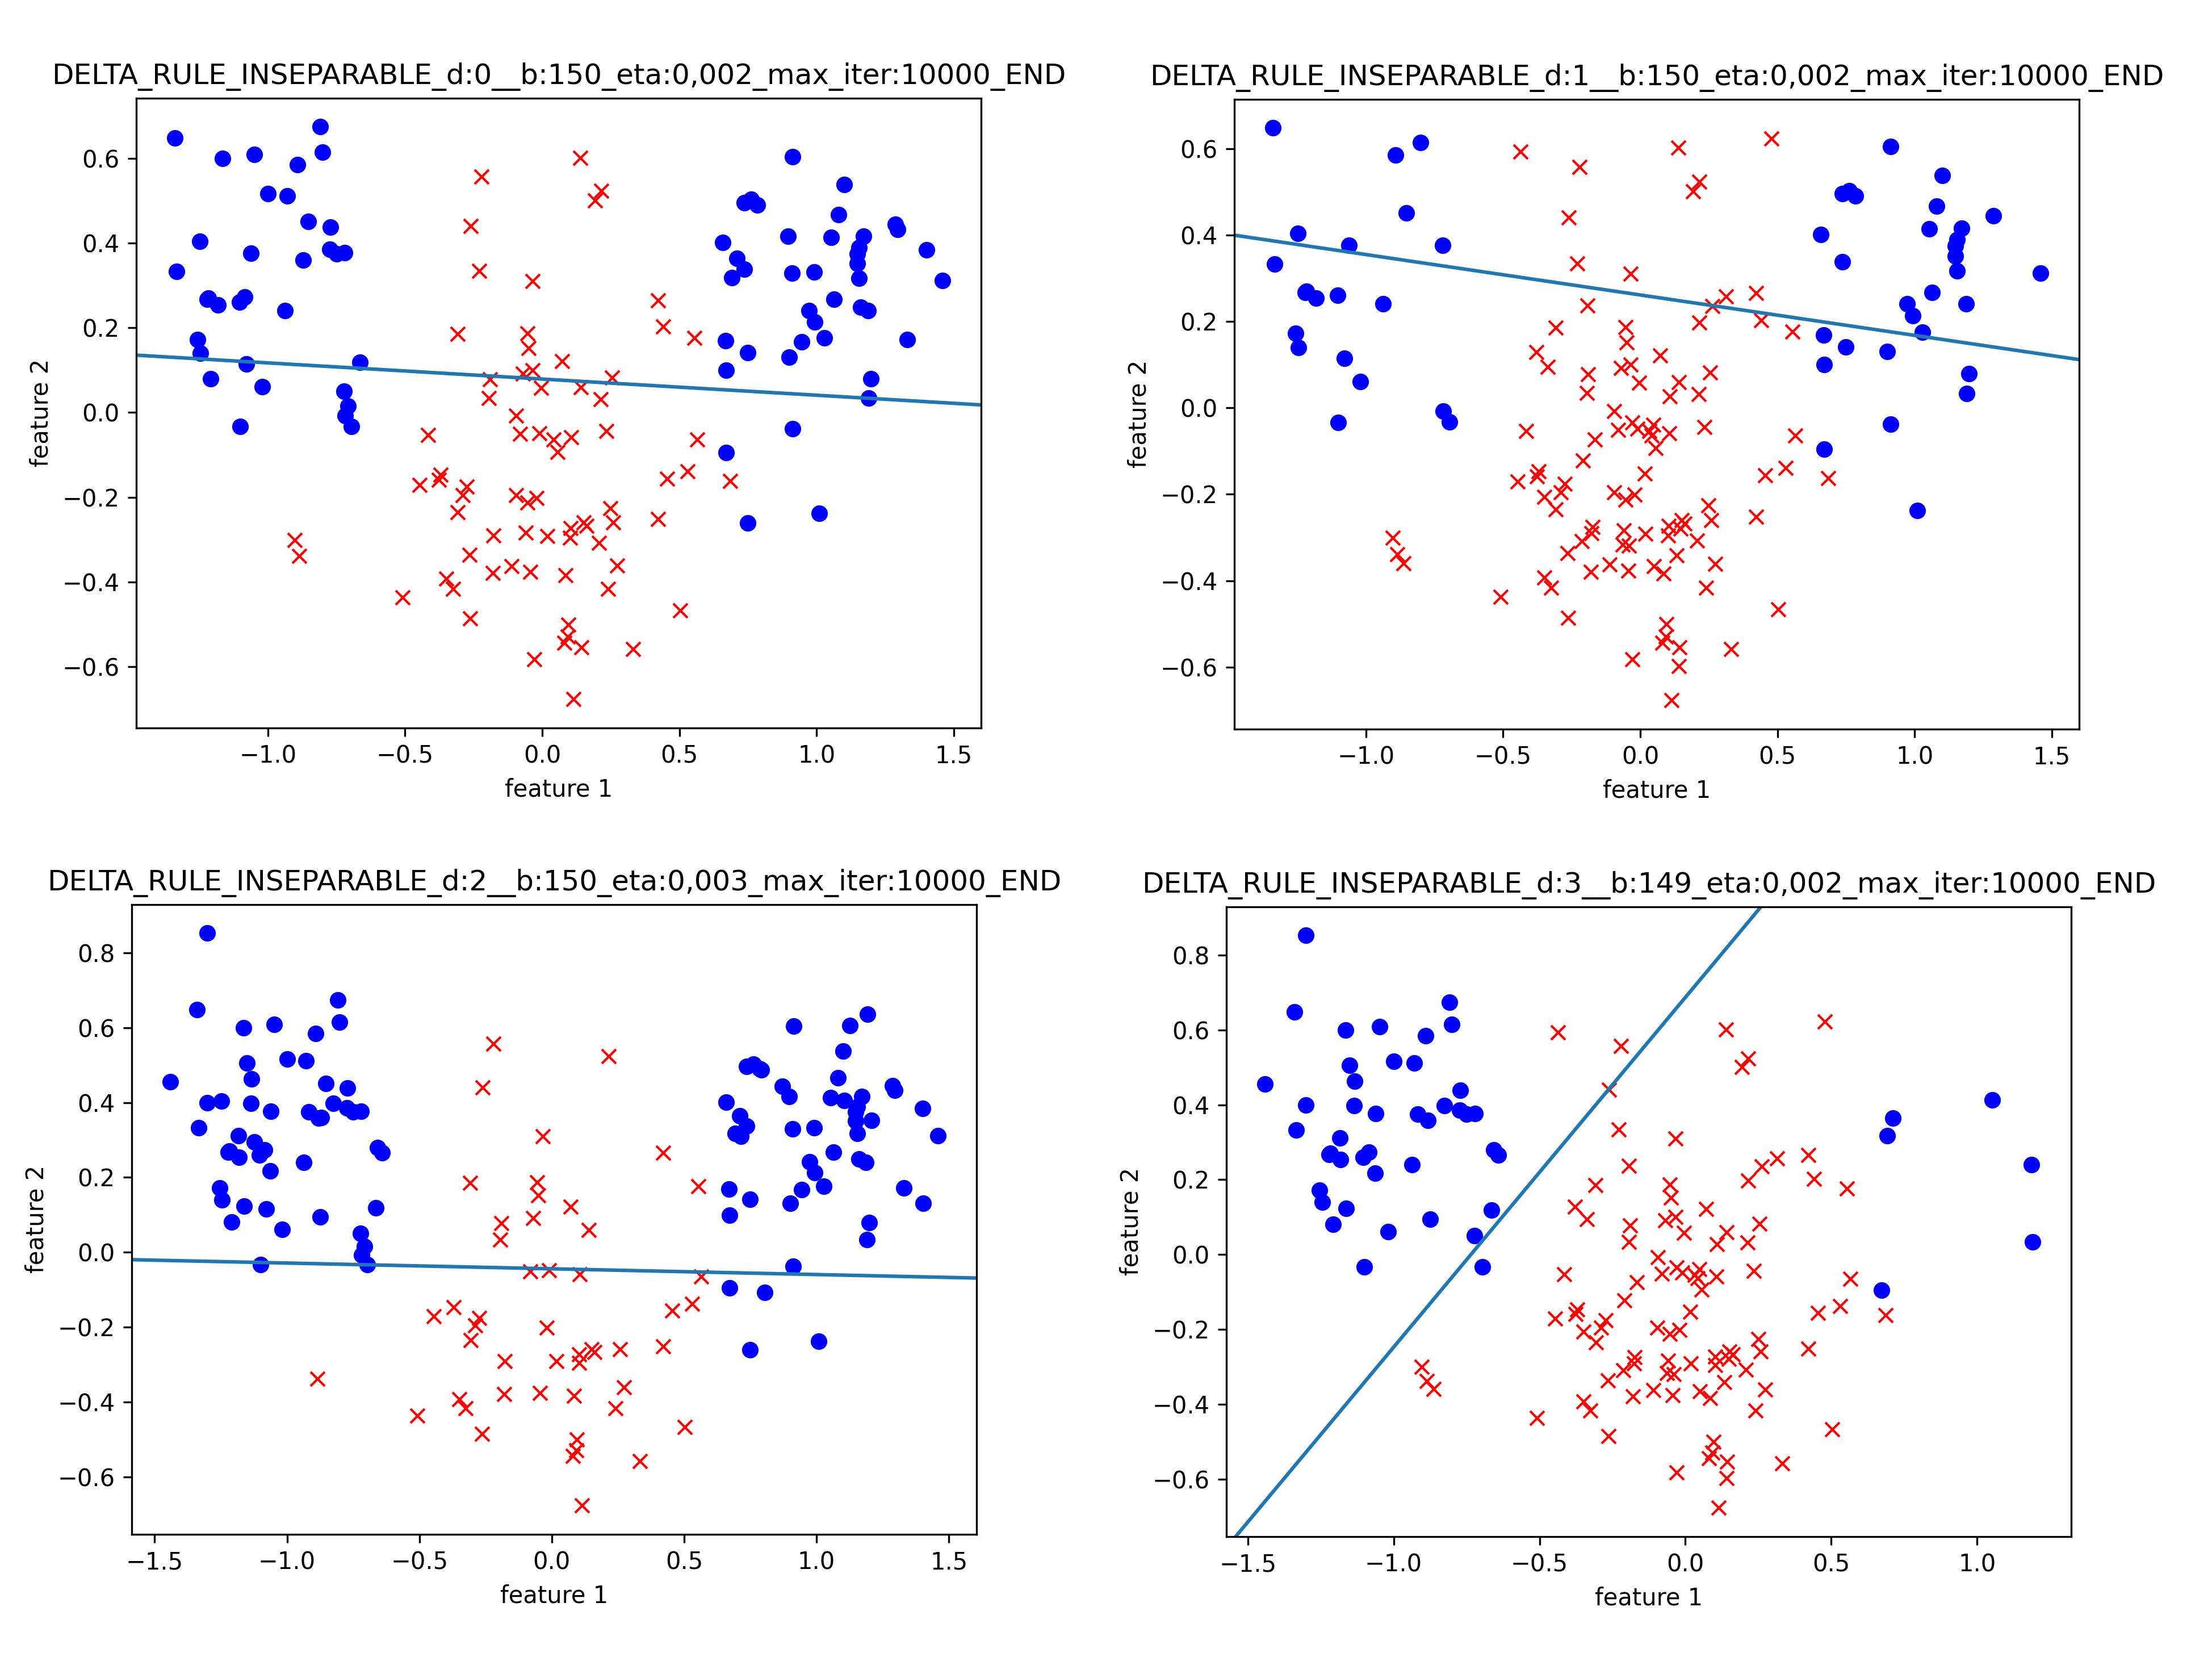
\includegraphics[width=10cm]{3.1.3_inseparable_datasets.png}
%	\caption{Decision boundaries for 4 subsampled datasets}
%	\label{fig:inseparable_datasets_lines}
%\end{figure}
\subsection{Classification and regression with a two-layer perceptron} % \textit{(ca.2 pages)}
\subsubsection{Classification of linearly non-separable data}
%\textit{It seems that one (decision boundary) or two plots (inclusing learning curves) should suffice. Build a story around the questions in the assignment. Include concise motivation for your findings and potential interpretations/speculations.}

Modifying the number of hidden nodes showed that at least 3 nodes are needed for the prepared two-class inseparable dataset for an accuracy of 100\%, which is to be expected having in mind the class distribution: one sigmoid function gives a line with threshold, two sigmoid functions with threshold give a more complex curve that, if observed, still cannot theoretically separate this dataset, so a more complex boundary must be created.

We created 4 subsets from the inseparable dataset (as described in section \ref{section_slp}) and divided the data into train and validation sets. Resulting decision boundaries for all 4 subsets are shown in Figure \ref{fig:d1234}.

\begin{figure}[h!]
	\centering
	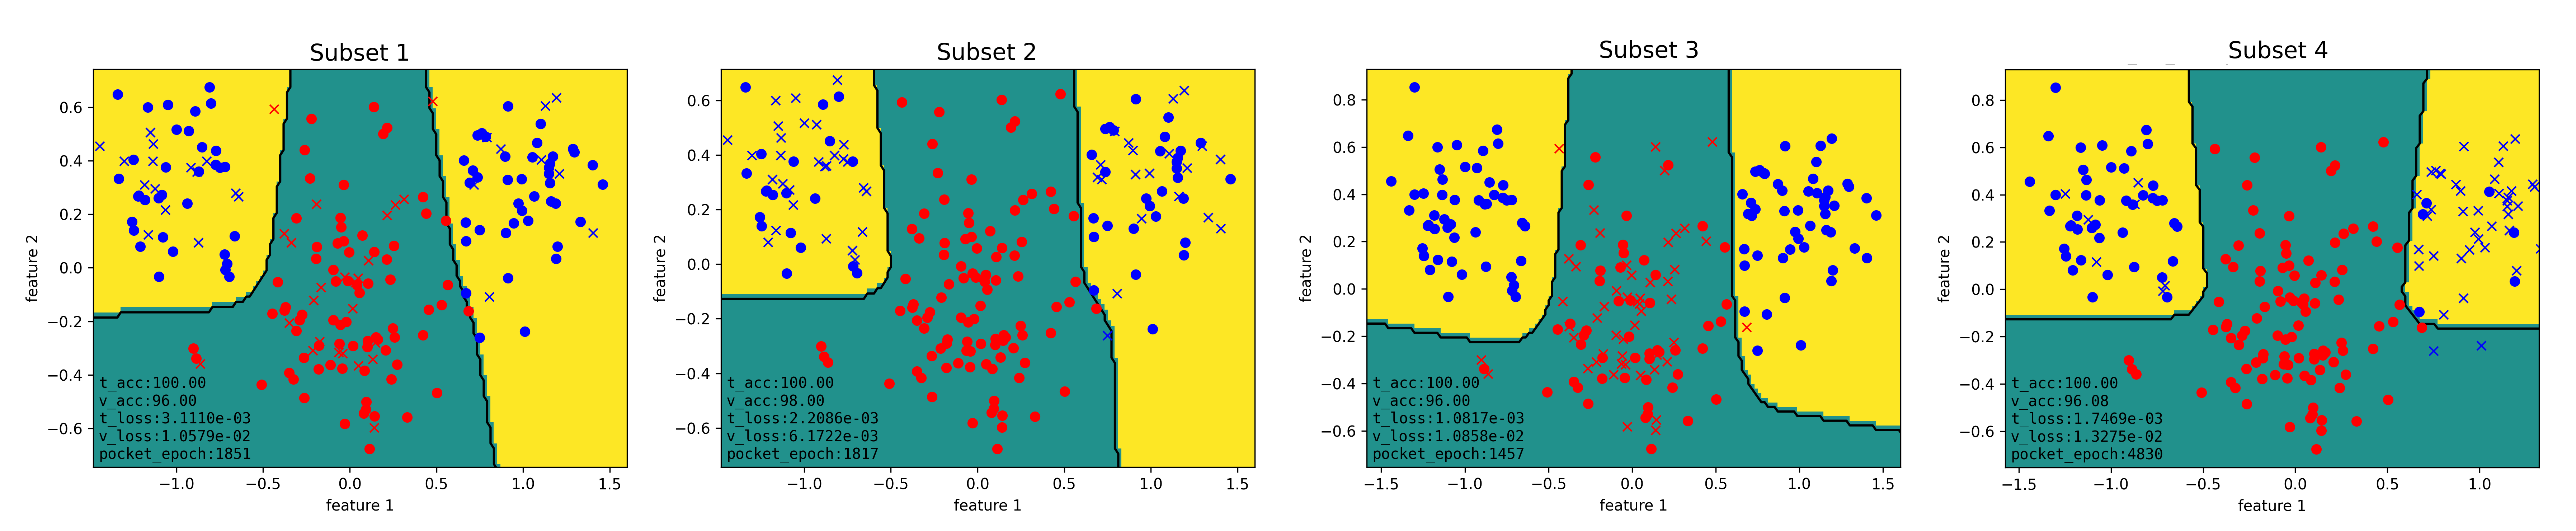
\includegraphics[width=12.5cm]{img/d1234.png}
% 	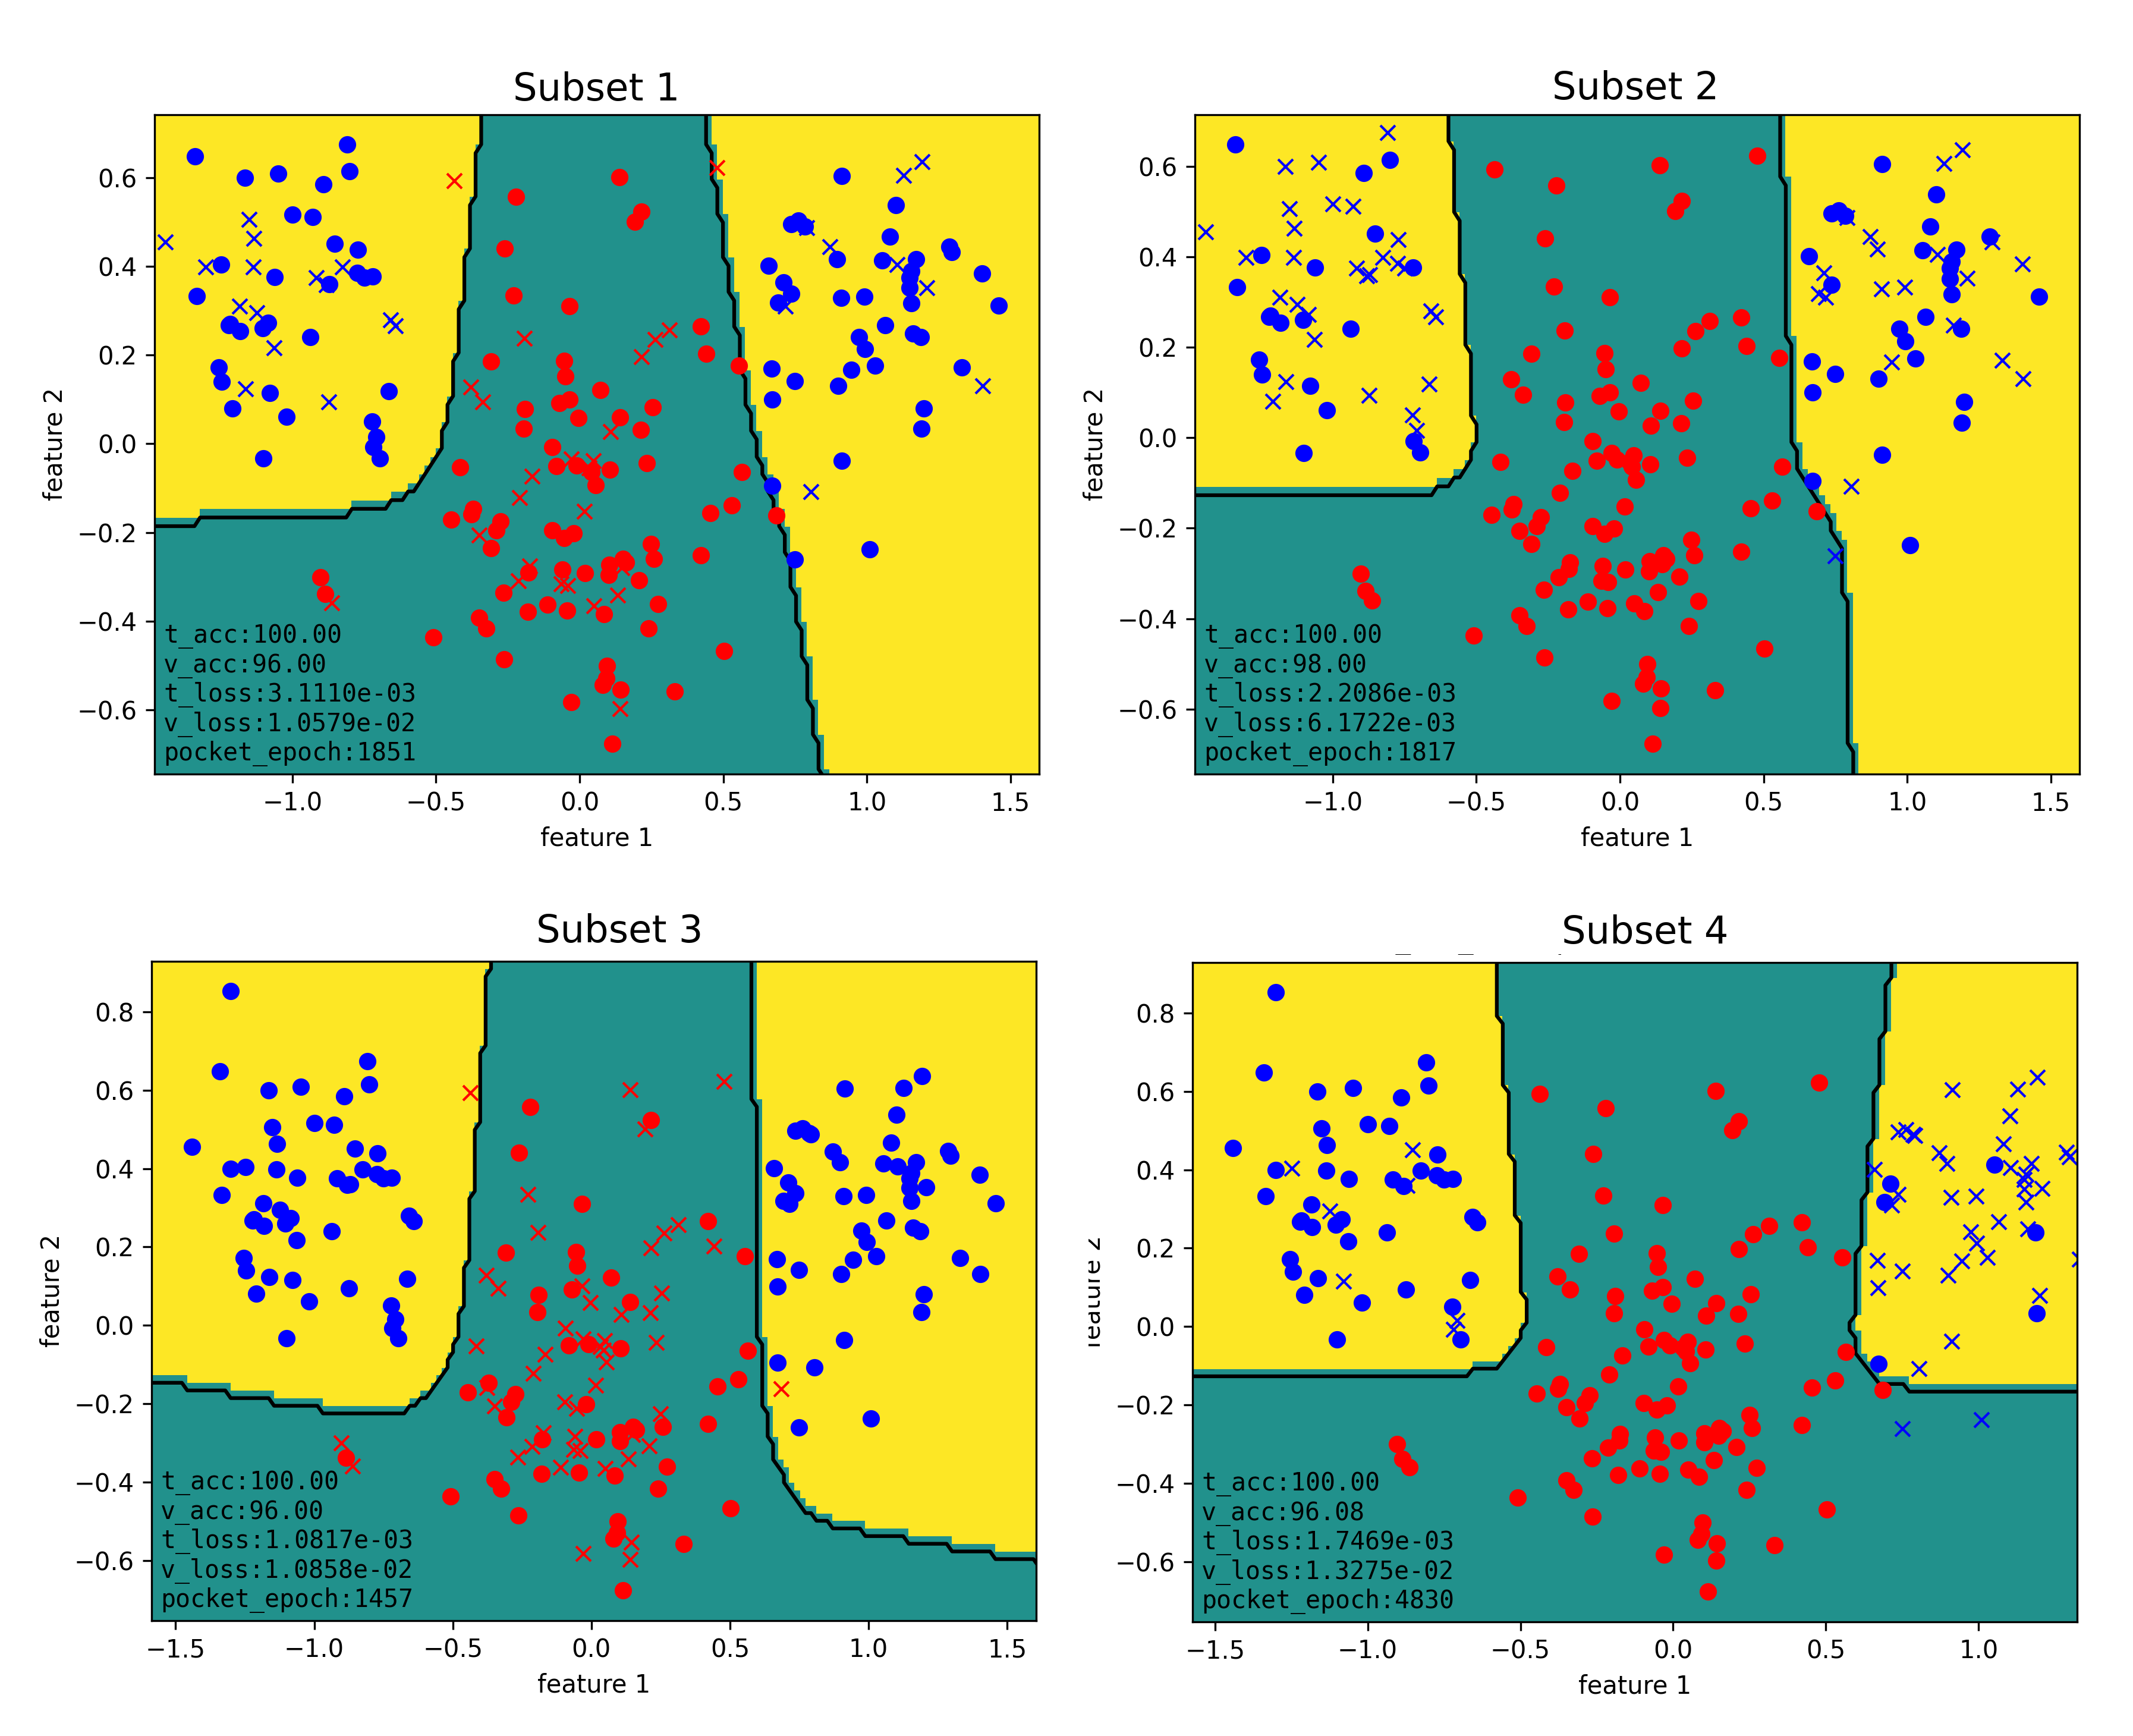
\includegraphics[width=10cm]{img/d1234_2.png}
	\caption{Multi layer perceptron results for all 4 subsets}
	\label{fig:d1234}
\end{figure}

The training error is consistently lower than the validation error, as shown in Figure \ref{fig:learning_curve}. Increasing the number of nodes lowers the training error as the network can adapt better to the data while the validation error rises as the network loses its generalisation capability. This rise in dissimilarity also depends on the dataset we use.

\begin{figure}[h!]
	\centering
	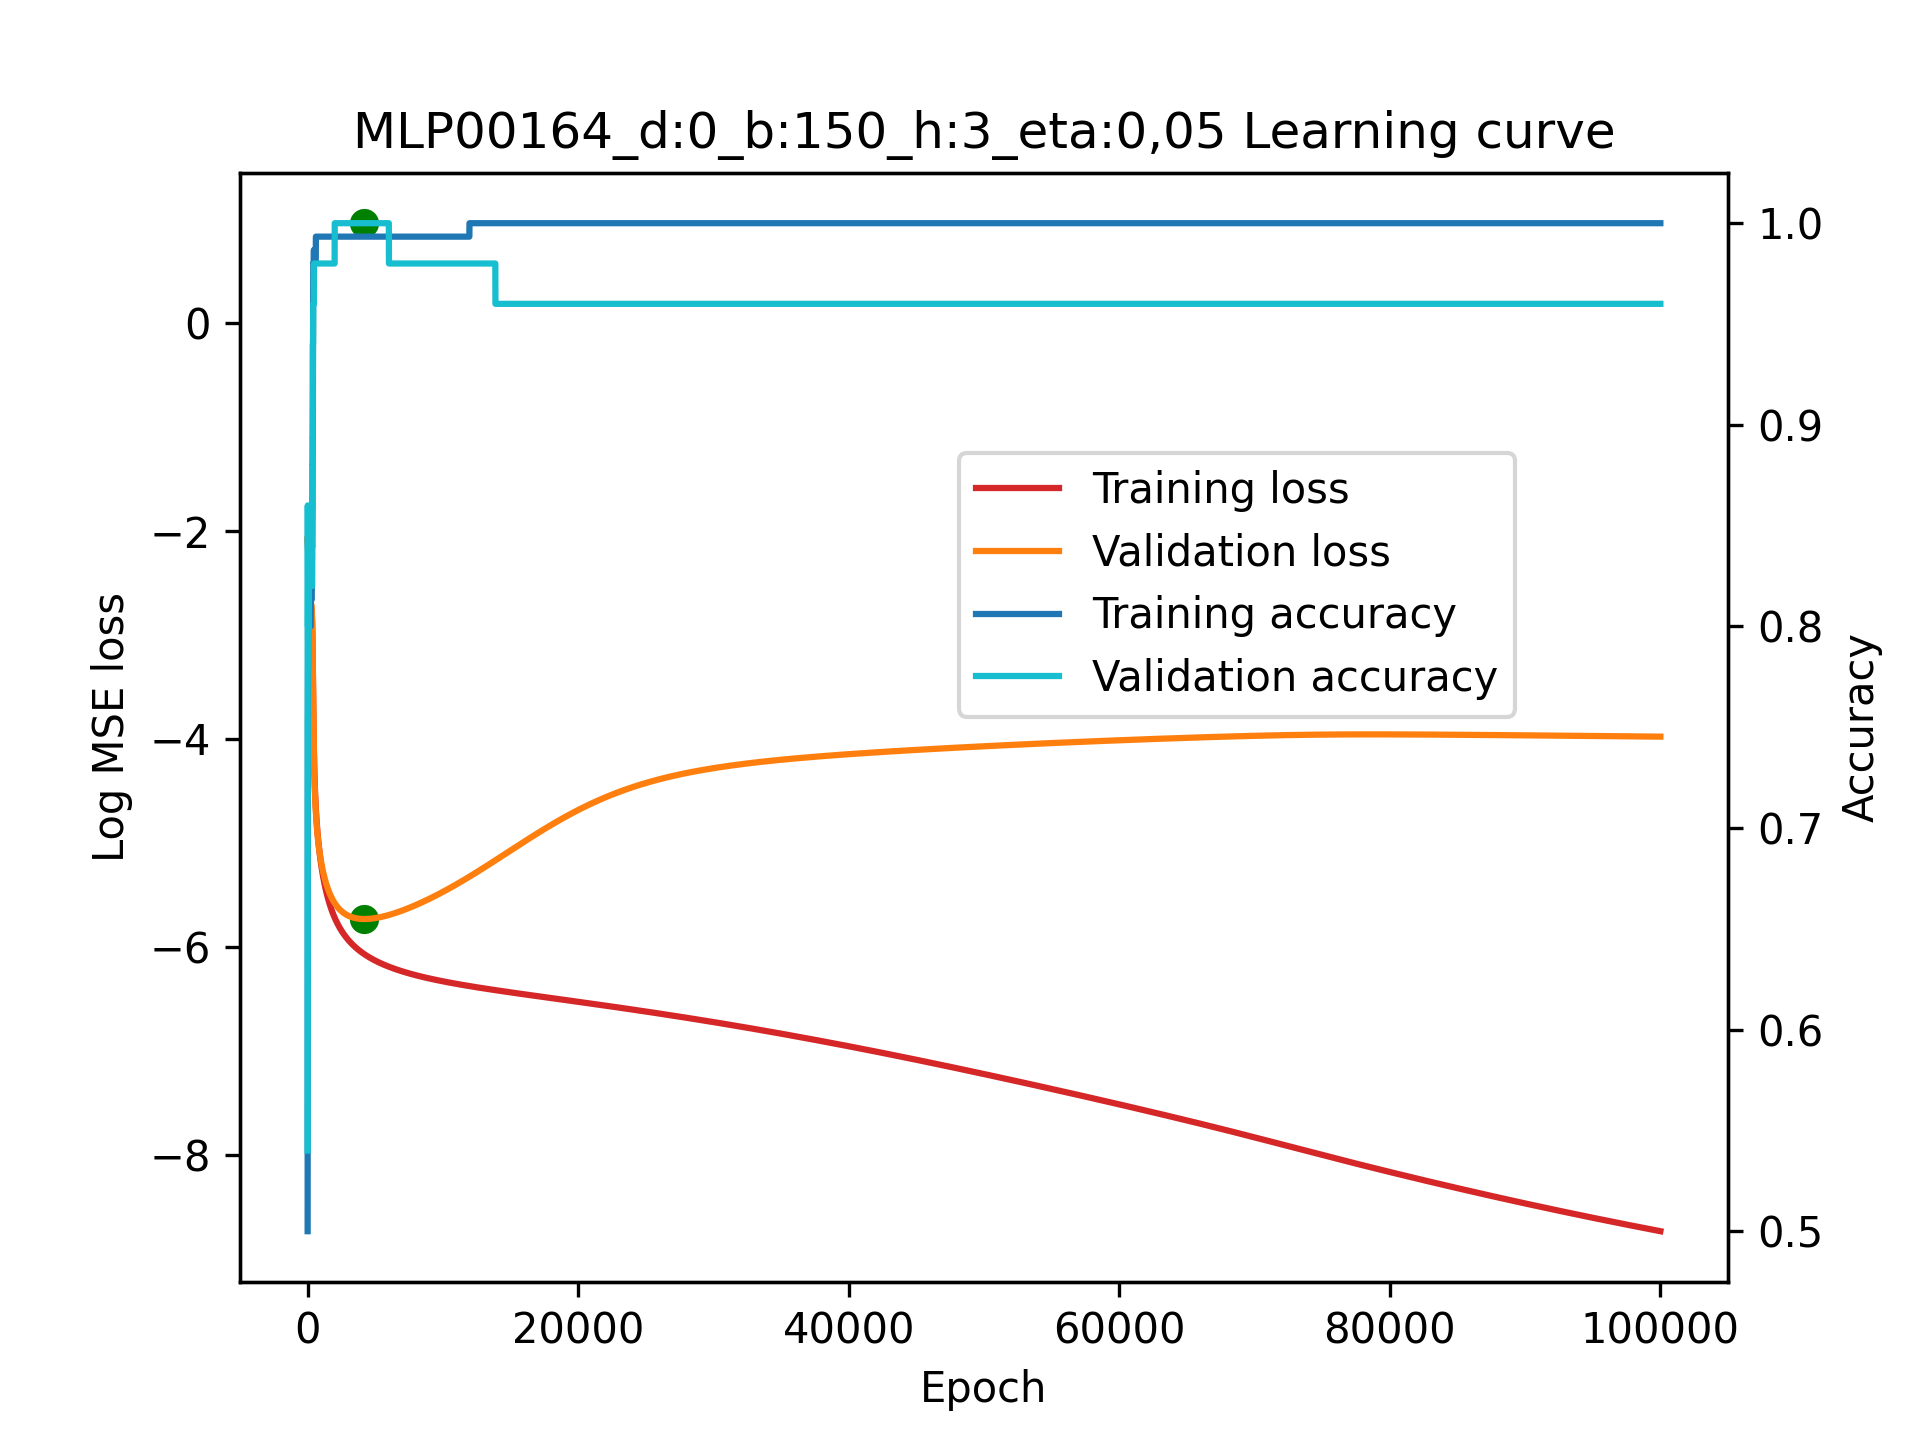
\includegraphics[width=8cm]{img/MLP00164_d:0_b:150_h:3_eta:0,05_learning_curve.png}
	\caption{Learning curve of Multi layer perceptron with 3 nodes in hidden layer. Batch learning with learning rate 0.05 was used on data subset 1.}
	\label{fig:learning_curve}
\end{figure}

Due to its noise, sequential learning is more robust to local minima and can therefore find a better solution than batch learning, lowering both training and validation errors. However, the noise can also negatively influence the performance of the network. In our experiments, there was no noticeable difference in performance with respect to using batch and sequential learning; they both achieved high validation accuracy, but sequential learning did so in a lower number of epochs. % in one configuration it was 10 times faster to reach ()

\subsubsection{The encoder problem}
%\textit{Here you do not really need any illustrations, this could be a very short section reporting on your experiments in line with the assignment questions.}

Given appropriate hyperparameters, an 8-3-8 network will always converge and map inputs to its three hidden nodes for the simple problem of mapping sparse "one out of 8" patterns. By looking into the hidden layer, we noticed the network used a binary encoding pattern to map $2^{3}=8$ input patterns. The weights of the first layer were positive for those inputs that should result in a $1$ in the hidden layer and negative for that which resulted in a $0$.

When using an 8-2-8 architecture, we noticed that the network still successfully maps all inputs, but now the hidden layer representation was different from a simple binary code. The representation is less interpretable but more efficient. % On the other hand, a 8-2-8 network was not successful when for same number of patterns that are not sparse, whereas 8-3-8 mapped them successfully.

As shown, multi-layer perceptron networks can be used to compress data. Given various inputs, the network learns a hidden and simpler representation thereof, and thus needs less memory to store the same data.

\subsubsection{Function approximation}
% \textit{This subsection requires plots to reflect intuitive visual interpretation of the results. Make sure that you condense information and avoid any excessive plotting. Here you might also need to incorporate some illustration of the network's generalisation performance or use a table to systematically report the results requested in the assignment.}

Multi-layer perceptrons are known for their ability to approximate an arbitrary continuous function. Here, we studied how a two-layer perceptron network approximated the bell shaped Gauss function.

By varying the number of nodes in the hidden layer from 1 to 25 as shown in Figure \ref{fig:mlp_nh}, we tested all models for validation loss on a 60\% data split of 1600 data points with different learning rates. We noticed that a low number of nodes, below 8, is not complex enough to lower the validation error as more complex models are capable of. We found that the best performance with respect to validation error is achieved for an architecture with 14 nodes in the hidden layer. Having more nodes than 20 starts to increase the validation loss again.

\begin{figure}[h!]
	\centering
	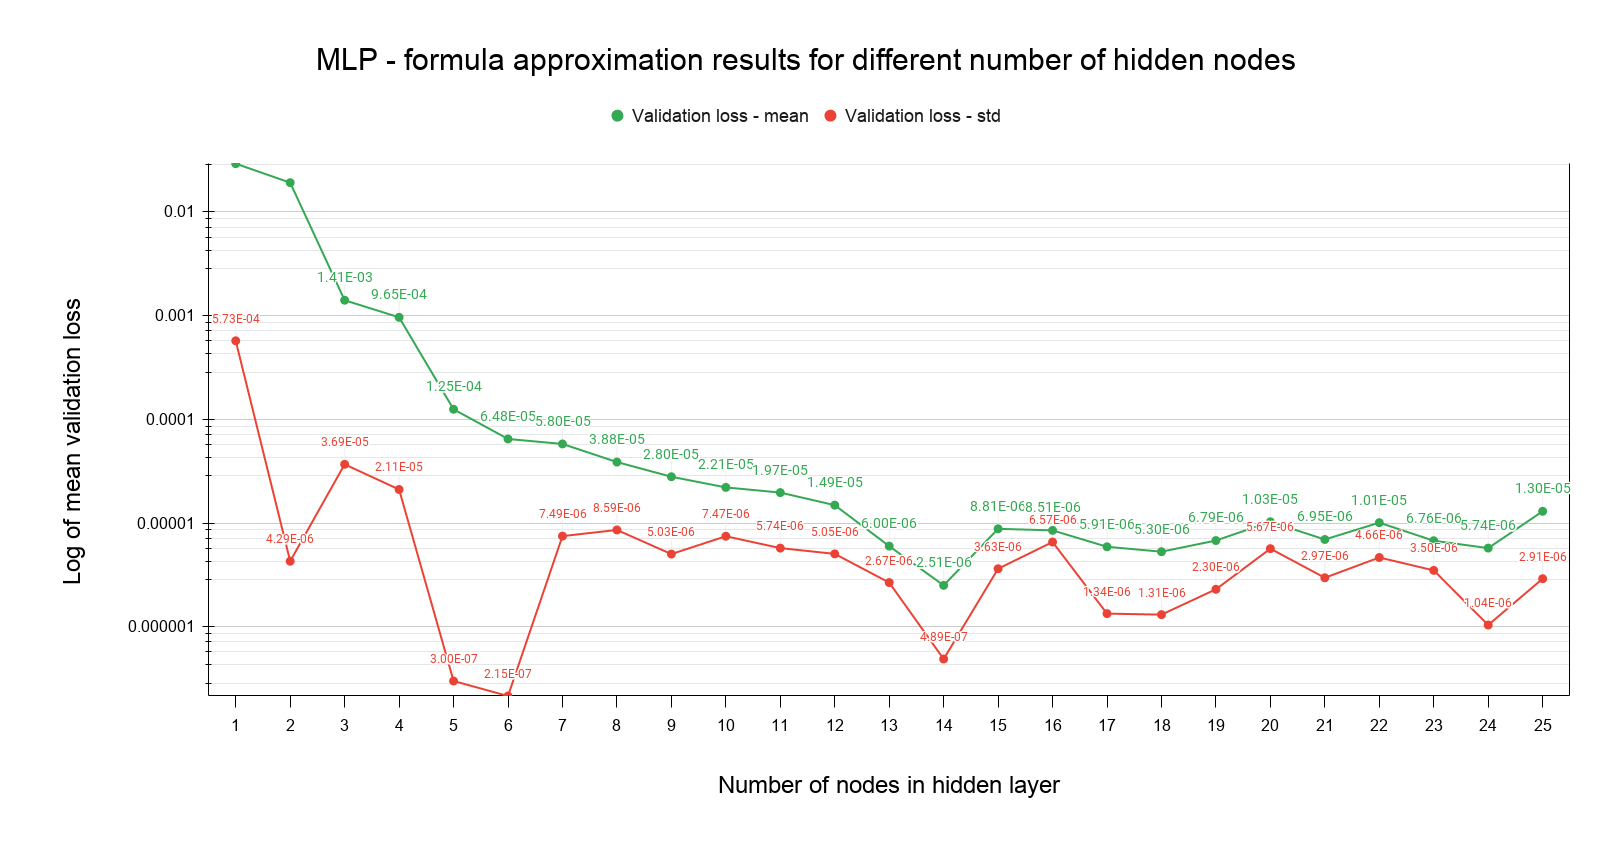
\includegraphics[width=9cm]{img/MLP - formula approximation results for different number of hidden nodes.png}
	\caption{Graph of validation loss in relation to number of nodes in hidden layer}
	\label{fig:mlp_nh}
\end{figure}

% 2. For the selected best model, run experiments with varying number of the training samples, e.g. from 80% down to 20% of all the dataset.
With the best model found, we run experiments with a varying number of training examples, with data splits from 80\% down to 20\%. We did not notice much difference in the results, which could be caused by the fact that the network is simple enough not to overfit.

% 3. For the best model, can you speed up the convergence withiout compromising the generalisation performance?
The convergence of the best model can be sped up using momentum, however this introduces yet another hyperparameter to tune.

% 4. A non-mandatory study, but interesting and didactical, could be to examine the behaviour of your two-layer perceptron with a varying number of hidden nodes in the presence of Gaussian noise, controlled by the variance, added to z variables (function outputs) in the training data subset.
% TODO?

\section{Results and discussion - Part II} % \textit{(ca.2 pages)}

%\textit{Here you do not have to introduce the problem or define Mackey-Glass time series, as you should focus on the results. You could divide them into two parts as the following two suggested subsections but you might as well keep your story under the main heading of Part II of the assignment. Importantly, always clearly state what network architecture you use, crucially with the number of hidden nodes, systematically report average results with various manipulations (regularisation etc.) and pay attention to differences between training, validation and test errors. Illustrating the outcome of your network predictions along with the original chaotic time series can also be very helpful. Finally, since you compare two- and three-layer architectures, make sure that you do not jump to any conclusions based on a small number of simulations unless you have statistically convincing evidence (when you compare the mean performance measures, their second moment is also relevant). In this part it may be particularly desirable to rely on tables.}

We generated the Mackey-Glass time series using starting conditions and formula given in the assignment, then we split it into three consecutive non-overlapping sets: train, validation and test (respectively 800, 200, 200 samples). Weight decay (L2 norm) regularization is used. Max number of epochs is $20000$ and we implemented early stopping such that if there is no improvement of at least $10^{-5}$ in the validation mean square error (MSE) for $50$ epochs, we stop the learning.

% For this assignment, we have used the 
%Mackey-Glass time series is used to evaluate performance of two-layer and three-layer perceptrons. The data was simply generated by using the starting conditions and sequentially calculating values using the iterative formula given in the assignment. Furthermore, the data was split into three consecutive non-overlapping blocks for training, validation, and testing using 800, 200, and 200 values, respectively. For the regularisation method we have used weight decay with the L2 norm. Early stopping is implemented in such a way that if improvement (by at least $10^{-5}$) in the validation mean square error (MSE) is not visible for 50 epochs the learning stops. Also, the maximum number of epochs allowed is capped at 20000.

\subsection{Two-layer perceptron for time series prediction - model selection, regularisation and validation}
Using learning rate of 0.1, as well as a medium regularization coefficient $\lambda = 0.1$, several two-layer perceptrons were tested, the results of which we can see in figure \ref{fig:learning_outcomes}. Each configuration was tested 10 times for larger certainty. We opted for the networks with 8 nodes in the hidden layer as those show the best results on the test set.

\begin{figure}[ht]
    \centering
    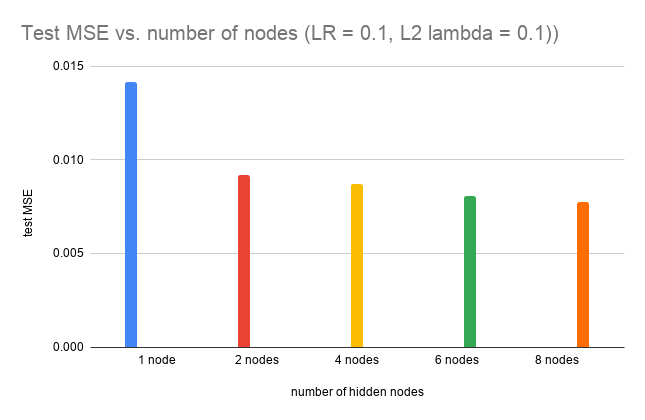
\includegraphics[width=.55\linewidth]{img/4_1_mse_bar.png}
	\caption{Test MSE for various network configurations}
	\label{fig:learning_outcomes}
\end{figure}

The impact of regularization on this network is less important that we would have expected. As seen in Figure \ref{fig:weight_histogram} few weights are drawn closer to zero. Our model might be too simple to overfit, plus we address the problem with early stopping. 

% Furthermore, we have tested the impact of regularization strength on the selected network. Generally, one could expect that the weights of a network with stronger regularization tend to be closer to 0, but this effect was not obvious in our case, probably due to the fact that our networks are too simple to have problems with overfitting and larger weights and also address these problems using early stopping. The described effect can to some extent be seen in figure \ref{fig:weight_histogram}.

\begin{figure}[hb]
	\begin{subfigure}{.5\linewidth}
		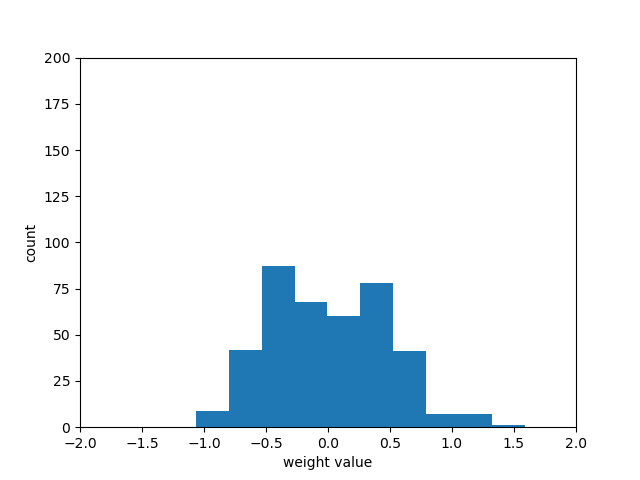
\includegraphics[width=.6\linewidth]{img/4_1_weight_histogram_0.png}
		\centering
		\caption{\small No regularization}
	\end{subfigure}
	\begin{subfigure}{.5\linewidth}
		\centering
		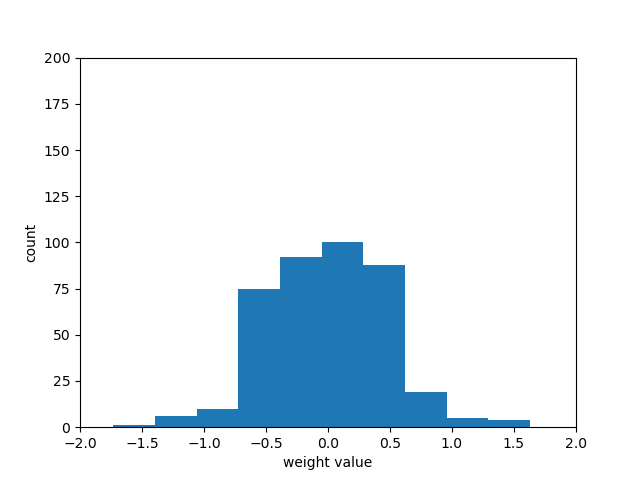
\includegraphics[width=.6\linewidth]{img/4_1_weight_histogram_0_1.png}
		\caption{\small L2 regularization $\lambda = 0.1$}
	\end{subfigure}
	\caption{Weight distributions}
	\label{fig:weight_histogram}
\end{figure}

% we have data for training an 8 hidden node network with a LR of 0.1 0.15 and 0.2; 0.15 shows best results
Finally, Figure \ref{fig:learning_process} shows an example of the learning process and the outputs of our selected network with 8 nodes in the hidden layer, a learning rate of 0.15 (which showed better results but slower convergence than 0.1) and an L2 weight decay with $\lambda = 0.01$. Those networks had an MSE of around 0.0036 on the test set which demonstrates their good capability of generalisation.

\begin{figure}[h!]
	\begin{subfigure}{.5\linewidth}
		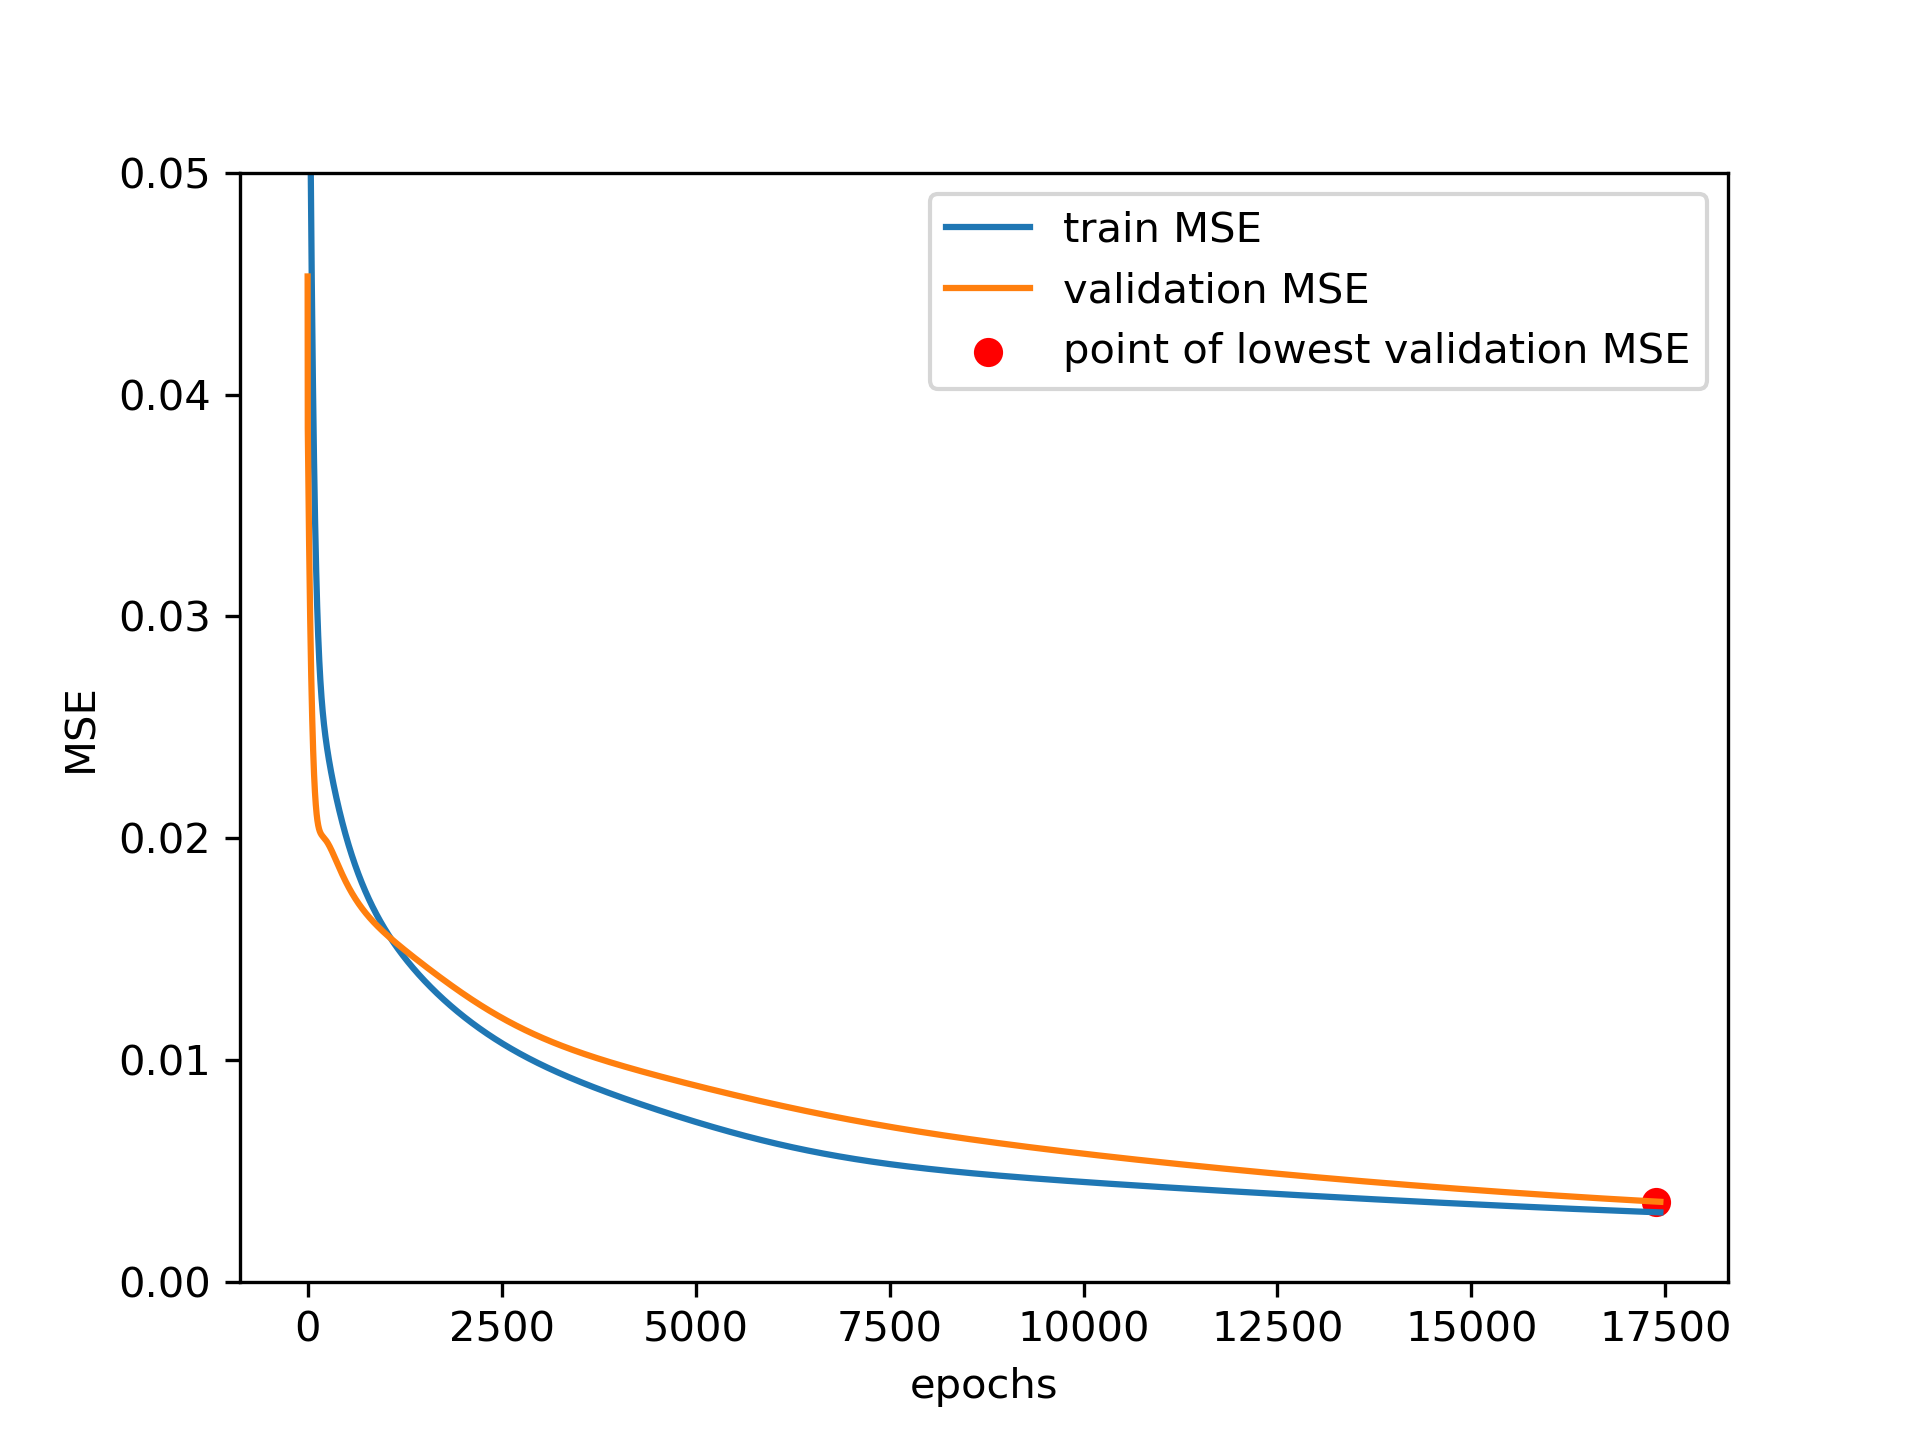
\includegraphics[width=170px]{img/4_1_learning_mse.png}
		\centering
		\caption{\small Learning process}
	\end{subfigure}
	\begin{subfigure}{.5\linewidth}
		\centering
		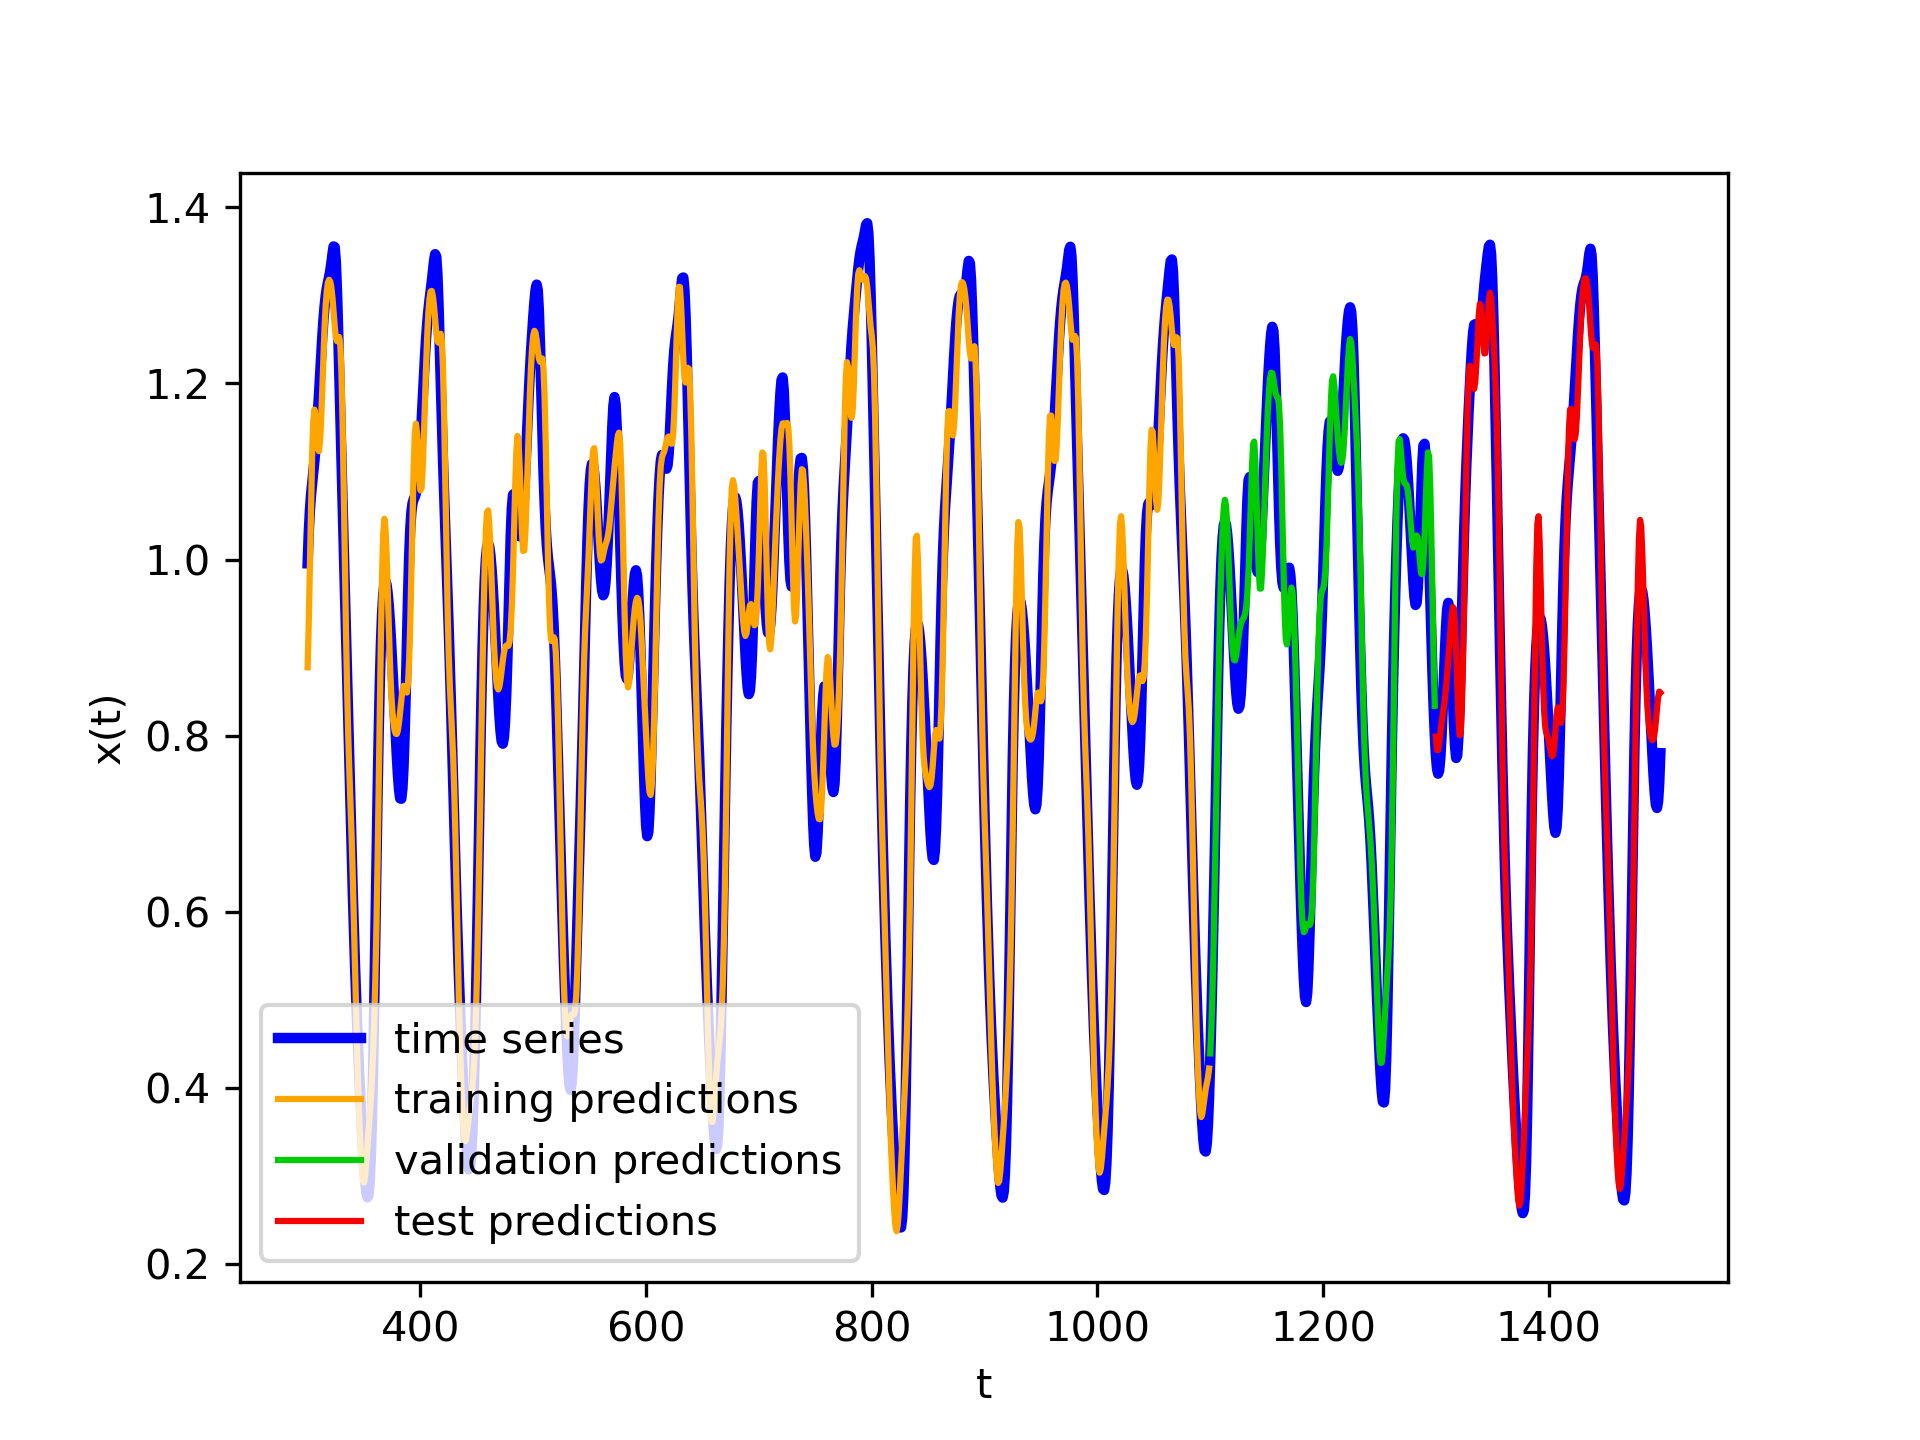
\includegraphics[width=170px]{img/4_1_predictions.png}
		\caption{\small Predictions after training}
	\end{subfigure}
	\caption{Learning process}
	\label{fig:learning_process}
\end{figure}

\subsection{Comparison of two- and three-layer perceptron for noisy time series prediction}
For this section zero-mean Gaussian noise was added to all target values.
%\begin{figure}[h!]
%	\begin{subfigure}{.5\linewidth}
%		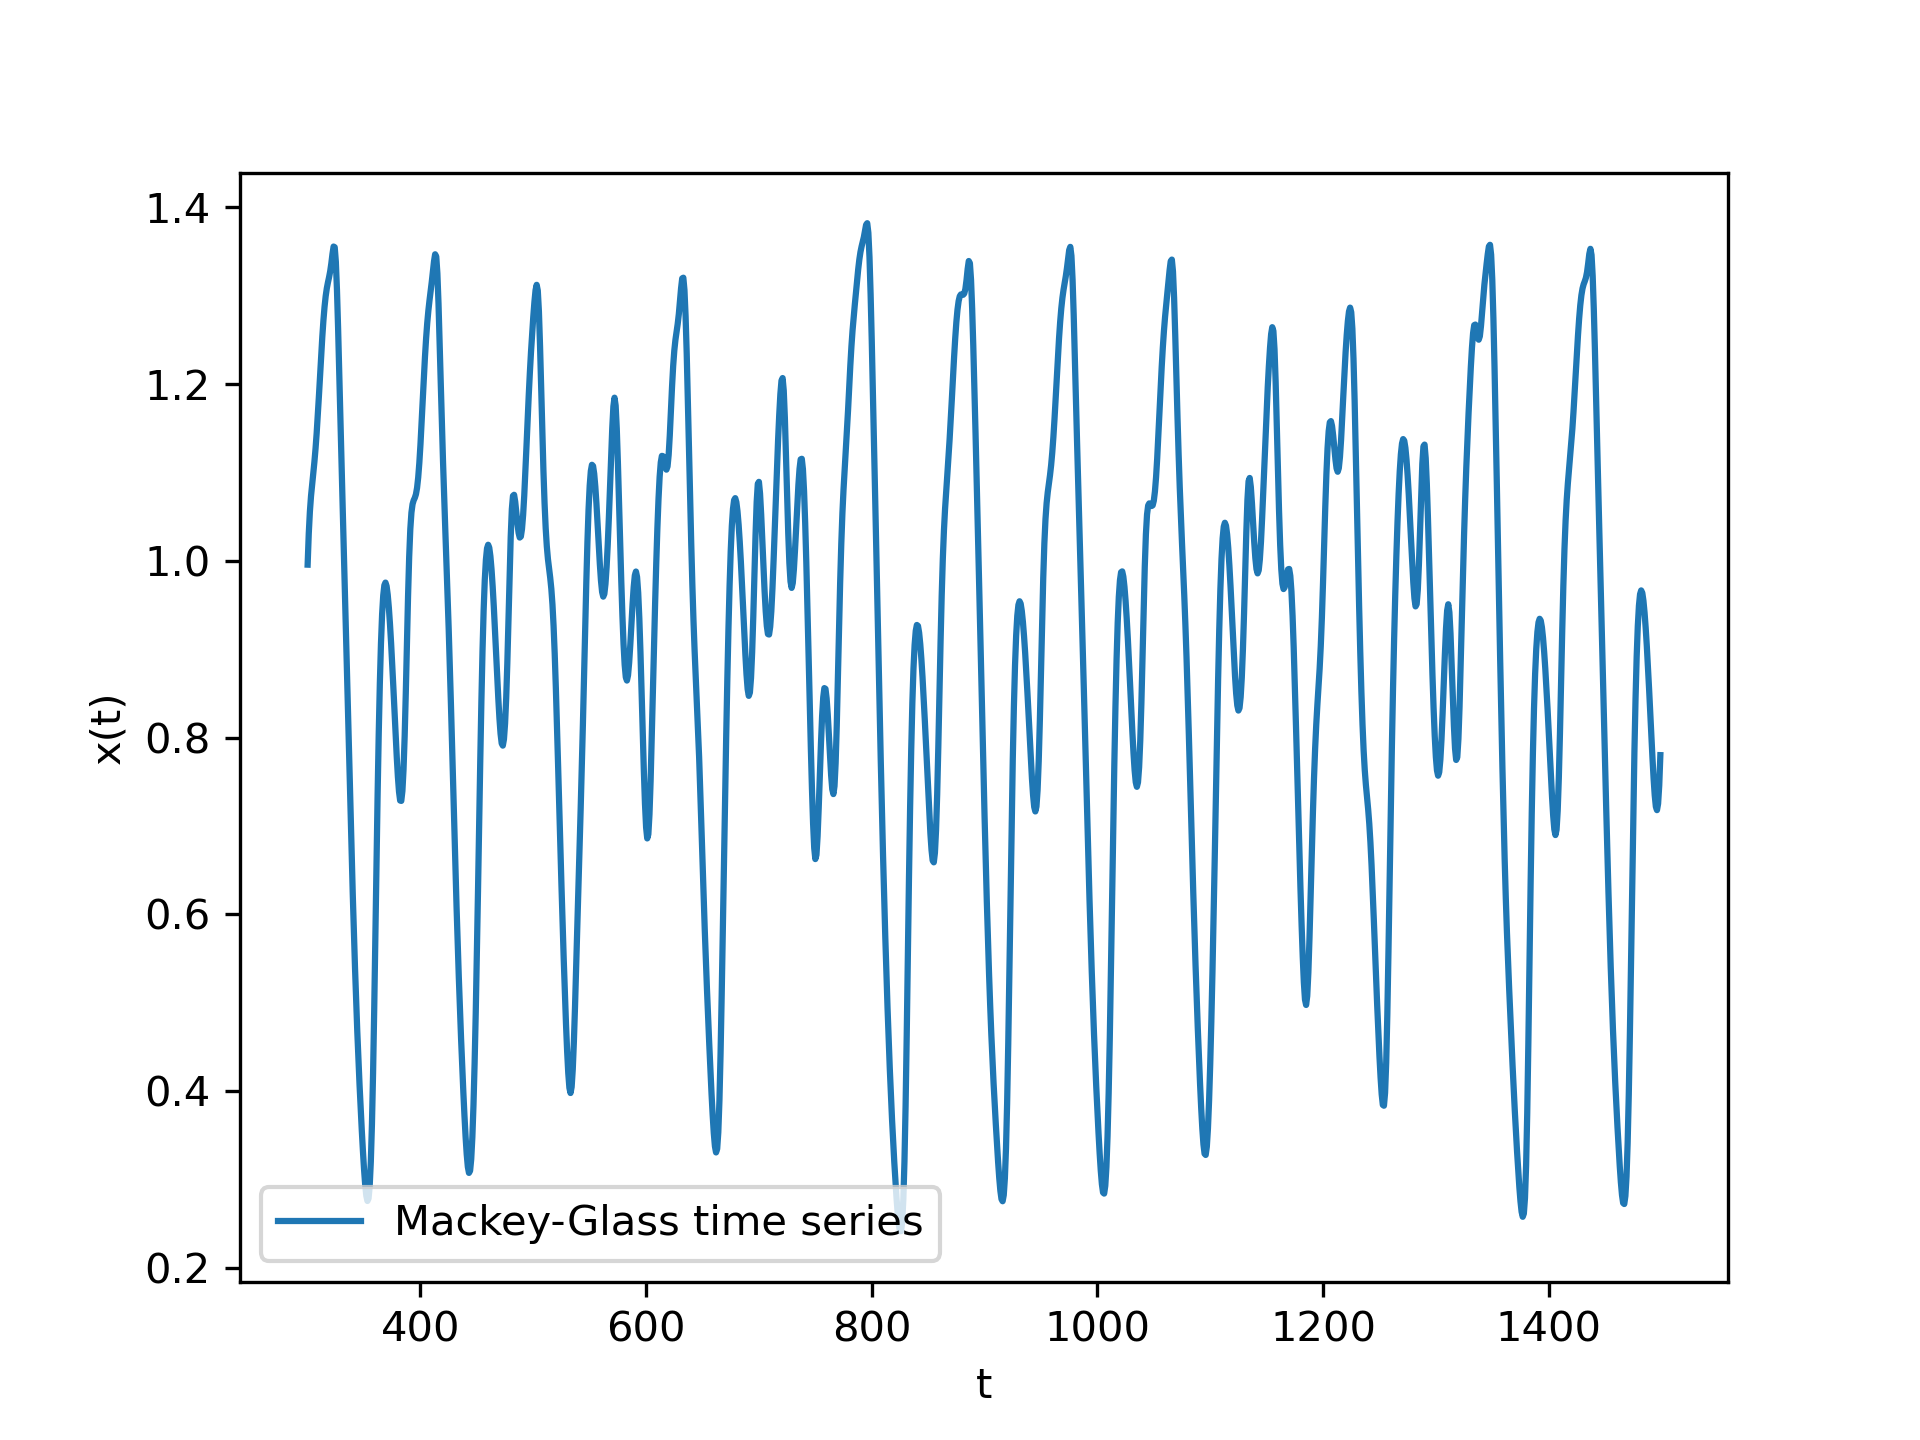
\includegraphics[width=170px]{img/4_2_series.png}
%		\centering
%		\caption{\small No noise}
%	\end{subfigure}
%	\begin{subfigure}{.5\linewidth}
%		\centering
%		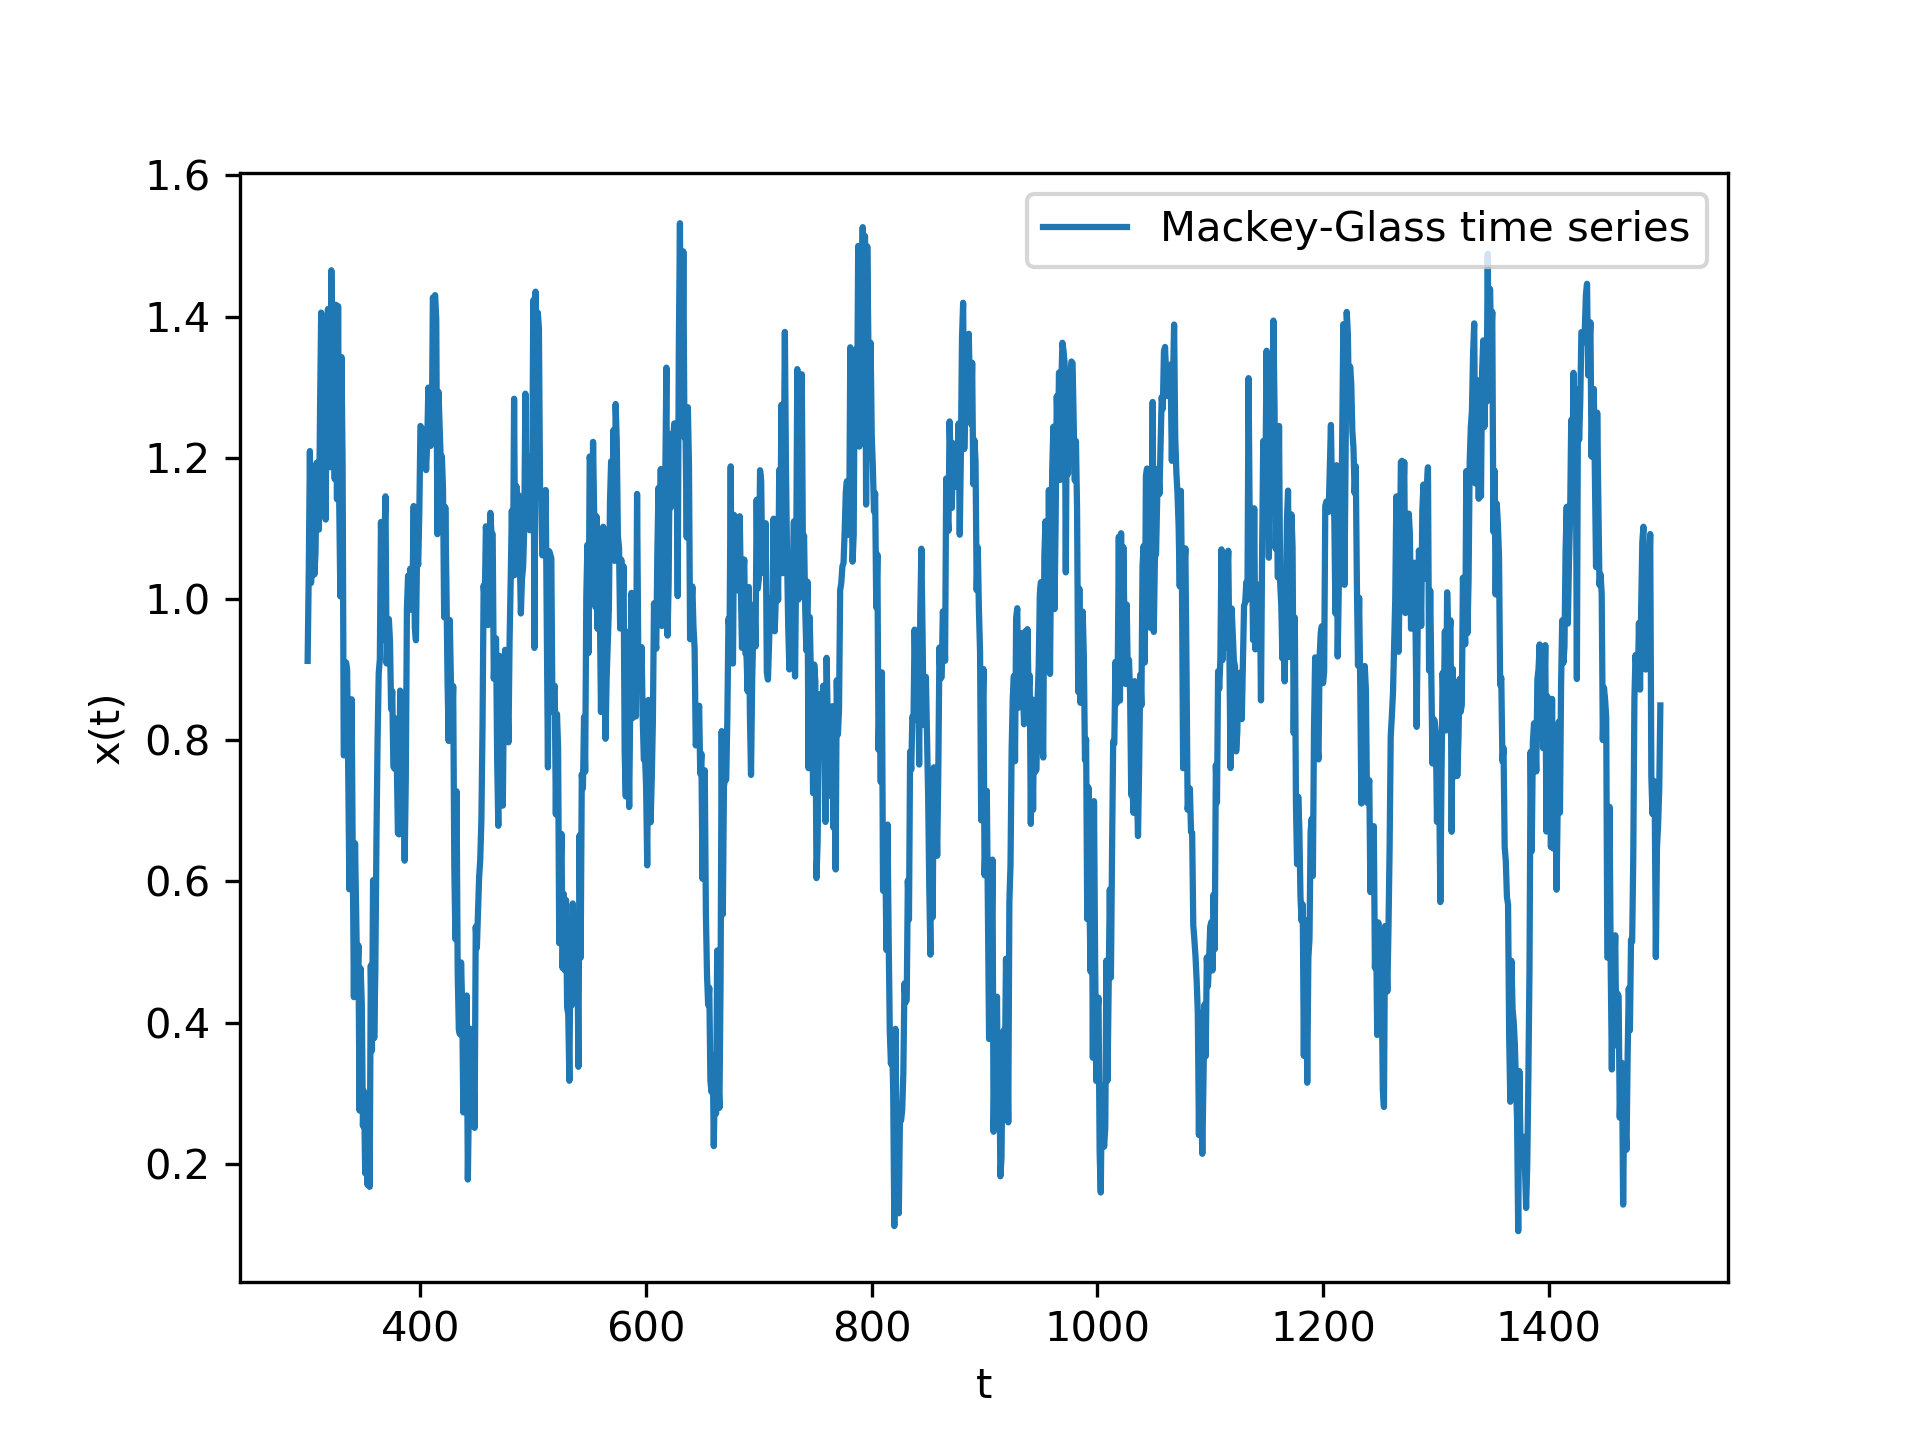
\includegraphics[width=170px]{img/4_2_noisy_series_0.09.png}
%		\caption{\small Noise with sigma = 0.09}
%	\end{subfigure}
%	\caption{Time series}
%	\label{fig:time_series}
%\end{figure}
Kept hyper-parameters for training were $\eta = 0.15$ and $\lambda = 0.1$

% For training we use a learning rate of 0.15 which showed the best results in the previous section of the assignment. We also use L2 weight decay with $\lambda = 0.1$ as in the previous tests.

We have tested a two-layer and a three-layer network with 8 nodes in each hidden layer and these have shown that training of the three-layer network takes about 50\% longer which is to be expected considering the sequential implications of the backpropagation algorithm.

The error on the all sets is larger when working with noisy data. This is to be expected as outputs are now more chaotic and less true to the underlying function; the irreducible error itself increases.

%\begin{figure}[h!]
%    \centering
%    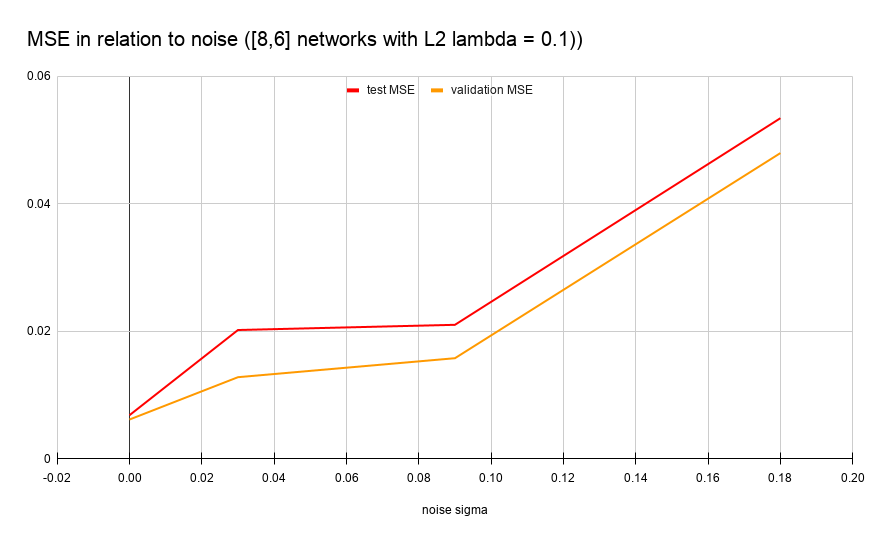
\includegraphics[width=250px]{img/4_2_noise_mse.png}
%	\caption{Mean MSE values in relation to noise levels for a network configuration}
%	\label{fig:weight_histogram}
%\end{figure}

As we add noise to the target values the network becomes more likely to overfit by learning noise instead of the underlying function. Furthermore, we are using a more complex model which can also cause overfitting. Thus, there is incentive to increase the strength of regularization methods to prevent these effects. $\lambda = 0.1$ showed the best results, 10 times higher than the $\lambda$ used with noiseless data. %(figure \ref{fig:regularisation_4_2})

%\begin{figure}[h!]
%    \centering
%    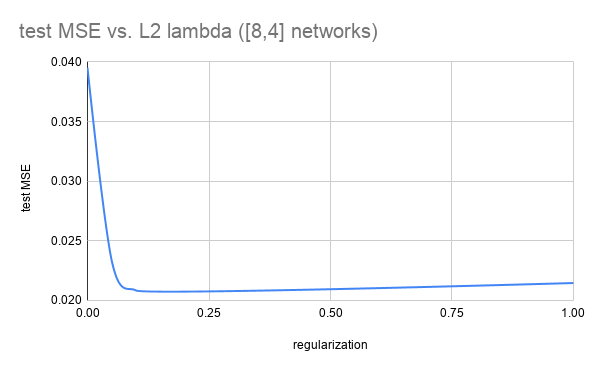
\includegraphics[width=250px]{img/4_2_regularisation.png}
%	\caption{Effects of regularization on the test MSE for a network with 8 nodes in the first, and 4 in the second hidden layer}
%	\label{fig:regularisation_4_2}
%\end{figure}

A network with 8 nodes in the first and 4 hidden nodes in the second hidden layer showed the best results for a noisy series with $\sigma = 0.09$ with a mean test MSE of 0.0208. The network with just one hidden layer and 8 nodes had a mean test MSE of 0.0201 which shows that, in this case, the network didn't benefit from an extra hidden layer.

\begin{figure}[h!]
	\begin{subfigure}{.5\linewidth}
		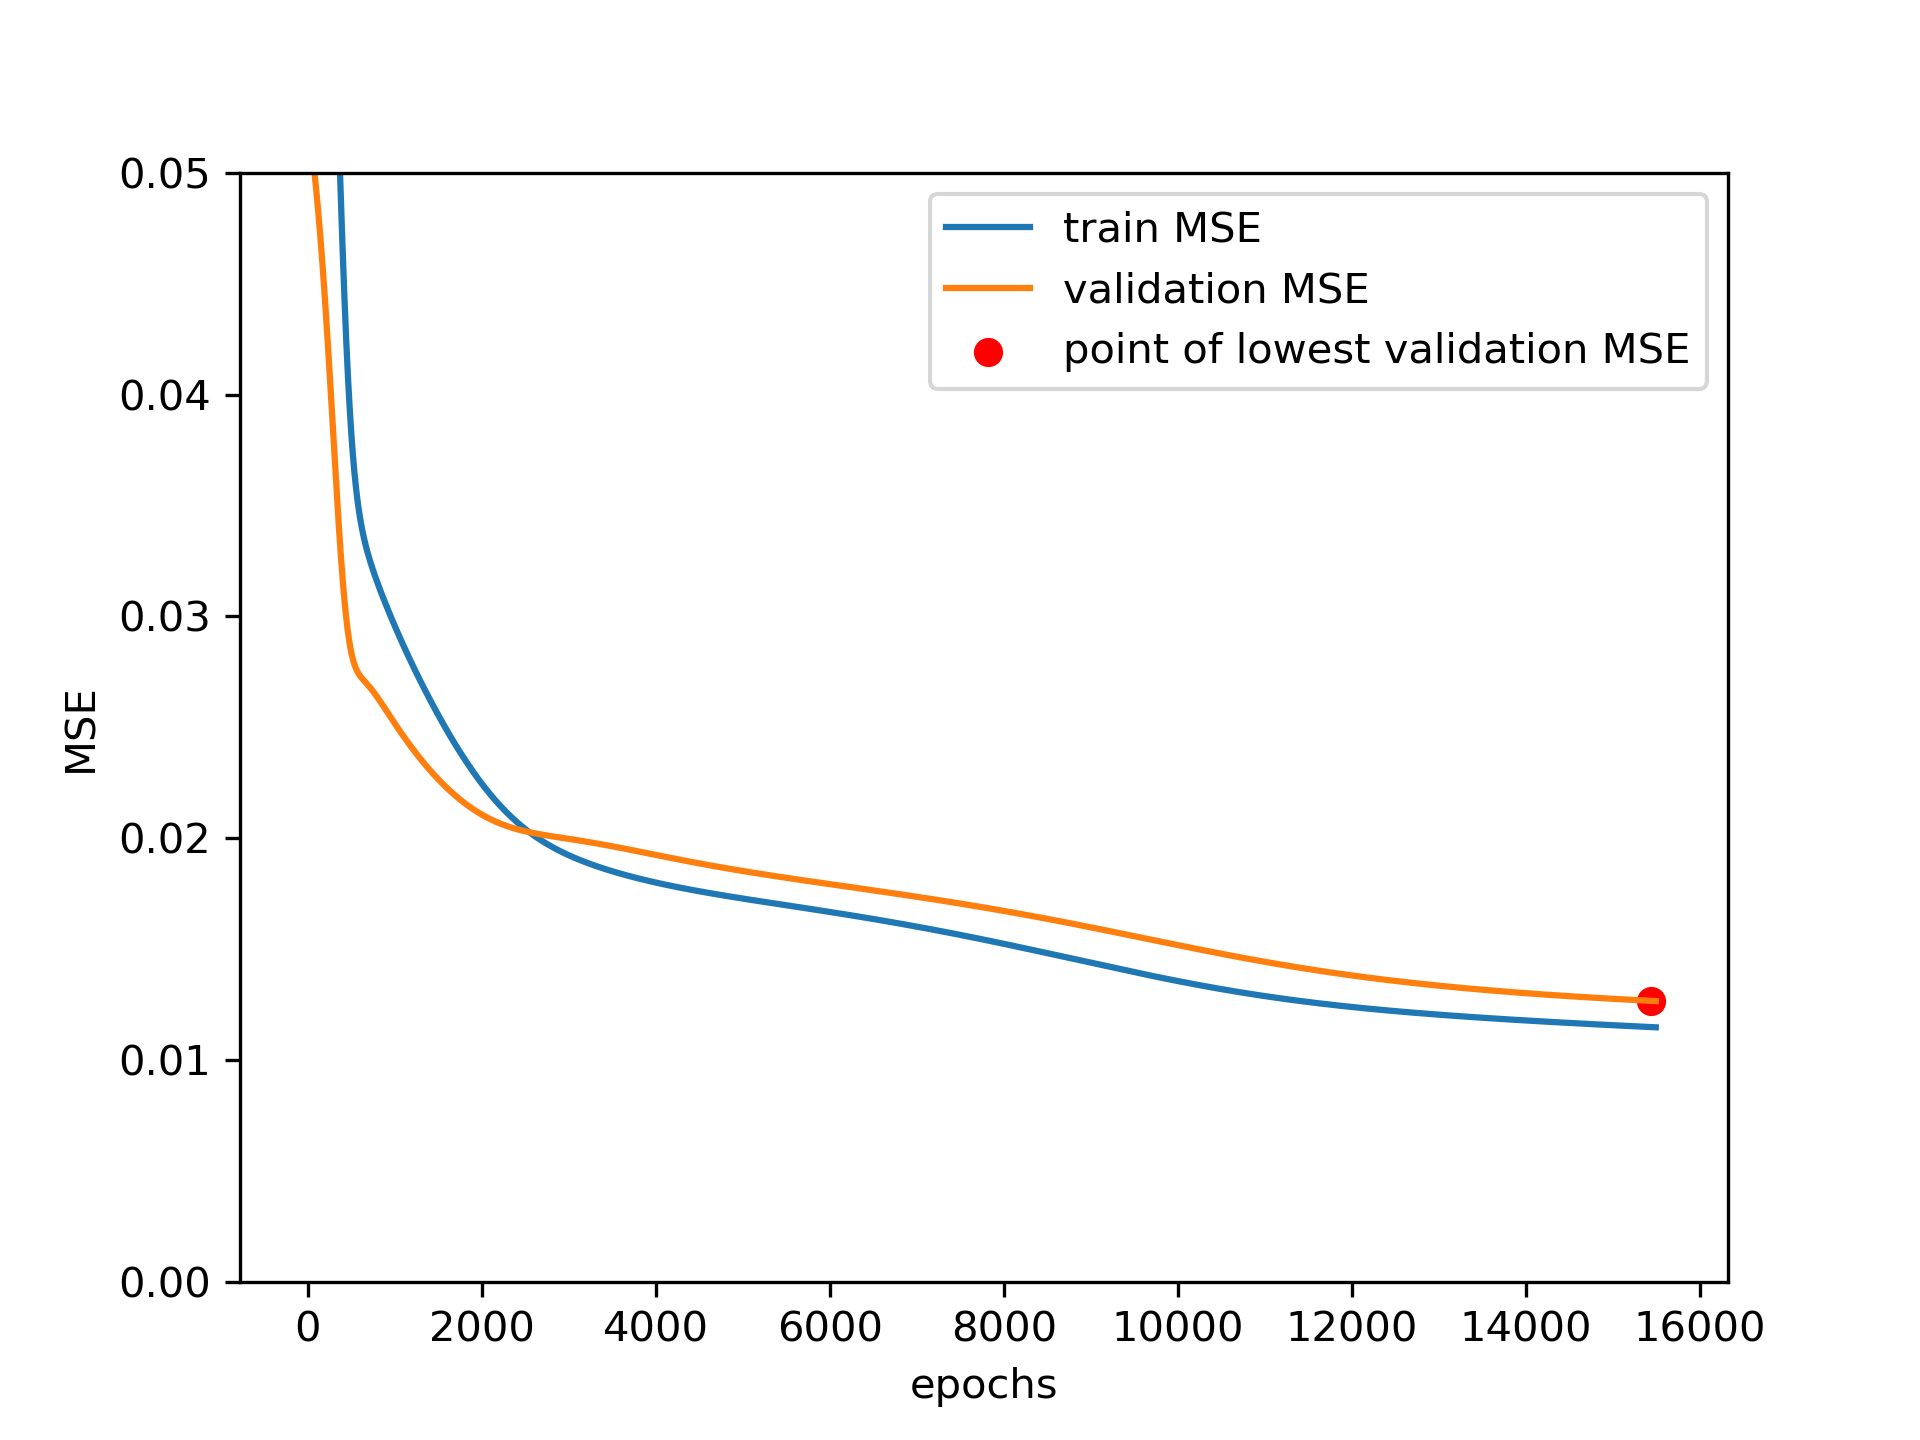
\includegraphics[width=170px]{img/4_2_learning.png}
		\centering
		\caption{\small Learning process}
	\end{subfigure}
	\begin{subfigure}{.5\linewidth}
		\centering
		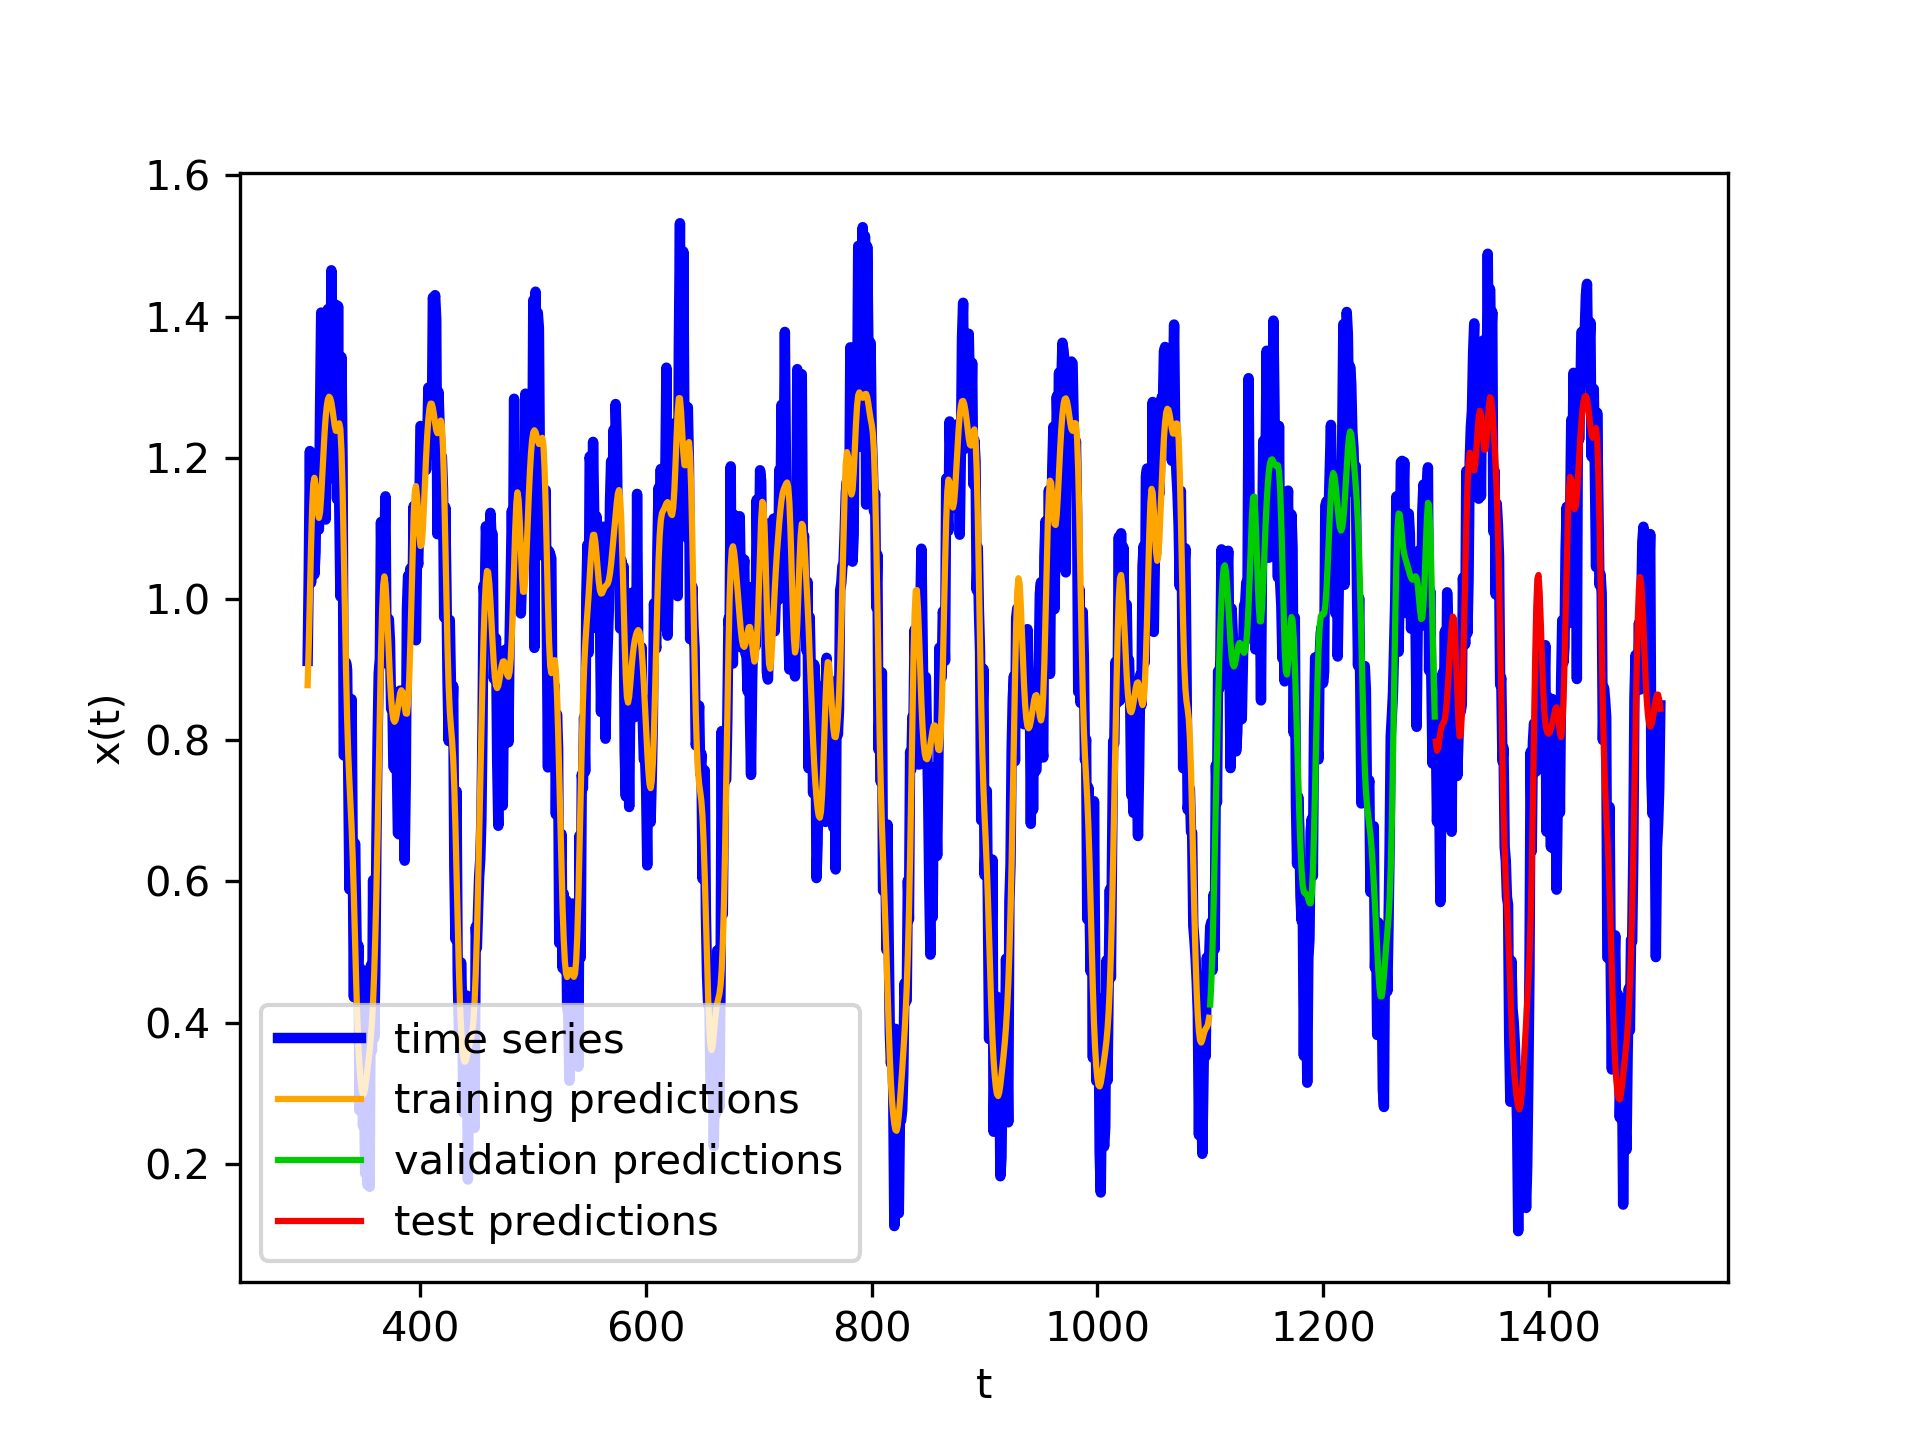
\includegraphics[width=170px]{img/4_2_predictions.png}
		\caption{\small Noisy time series and all predictions}
	\end{subfigure}
	\caption{Typical performance of a network for 0.09 noise sigma }
	\label{fig:learning_process}
\end{figure}

\section{Final remarks} % \normalsize{\textit{(max 0.5 page)}}
% \textit{Please share your final reflections on the lab, its content and your own learning. Which parts of the lab assignment did you find confusing or not necessarily helping in understanding important concepts and which parts you have found interesting and relevant to your learning experience? \\
% Here you can also formulate your opinion, interpretation or speculation about some of the simulation outcomes. Please add any follow-up questions that you might have regarding the lab tasks and the results you have produced.}
The lab was quite difficult in terms of creating all the needed software support and running various tests, but overall very useful for observing the effects of various hyperparameters and methods used in artificial neural network. It was insightful as a practical demonstration of theoretical concepts and showed that artificial neural networks actually do work, and do so well in both regression and classification problems.
\end{document}

https://www.overleaf.com/project/5f55ee1a0fc44d0001067a79